%
%  Dyerlab Documentation: gstudio vignette
%
%  Created by Rodney Dyer on Wed 11 January 2012.
%
\documentclass[letterpaper,twoside,openany]{book}
\usepackage[margin=0.75in]{geometry}
\usepackage[T1]{fontenc}
\usepackage[scaled=0.8]{helvet}
\renewcommand*\familydefault{\sfdefault}
\usepackage{kmath,kerkis}
\usepackage{parskip}
\usepackage{makeidx}
\usepackage{Sweave}
\usepackage{amssymb}
\usepackage{amsmath}
\usepackage{curves}
\usepackage{color}
\definecolor{header}{RGB}{79,129,189}
\newcommand{\Heading}[1]{\textcolor{header}{\Large \bfseries #1}}

\title{The \texttt{gstudio} Package}
\author{Rodney J. Dyer\\Department of Biology\\Virginia Commonwealth University}
\date{\today}

%\VignetteIndexEntry{gstudio Overview}


\begin{document}
\pagestyle{empty}
\maketitle

\frontmatter




\chapter{Preface}

This document is intended to be a more in-depth overview of the functionality contained in the \texttt{gstudio} package.  This package is released under the GPL so if you have particular additions you would like to make to it, feel free to submit them to rjdyer@vcu.edu.

\tableofcontents


\mainmatter

\chapter{Getting Genetic Data Into R}

\section{Synopsis}

Here you will learn to get genetic data files into the R environment using the \texttt{gstudio} package.  This package was designed to handle marker-based genetic data (e.g., not sequences \emph{per se} though it can use SNP's and haplotypes) as well as additional data that is typically collected along with individuals.  

To get started, first import the \texttt{gstudio} package as:

\begin{Schunk}
\begin{Sinput}
> require(gstudio)
\end{Sinput}
\end{Schunk}



\section{The \texttt{Locus} Class}

The locus class is the fundamental class that handles marker-based genetic data.  At present it can handle dominant and co-dominant marker types at any ploidy level.  Internally, alleles are stored as a \texttt{character} vector and by default they are not sorted so that the alleles will be presented in the order that you import them (e.g., a \texttt{3:1} locus instead of a \texttt{1:3} locus).  I do not sort these because it may be necessary to know the phase of the alleles in a locus and sorting them would remove that information.  If you abhor the sight of a genotype \texttt{3:1} then sort it earlier and then try to figure out why you have this affliction.  

\begin{Schunk}
\begin{Sinput}
> loc1 <- Locus( c(120,122) )
> loc1
\end{Sinput}
\begin{Soutput}
120:122 
\end{Soutput}
\begin{Sinput}
> loc2 <- Locus( c("A","T") )
> loc2
\end{Sinput}
\begin{Soutput}
A:T 
\end{Soutput}
\end{Schunk}

Note, that internally the alleles are translated into \texttt{character} objects.  In all the functions dealing with alleles both \texttt{integer} and \texttt{character} arguments are accepted.  There are several methods associated with the \texttt{Locus}, the main ones that you will be working with are shown below by example.  See \texttt{help("Locus-class")} for a complete discussion.


\begin{Schunk}
\begin{Sinput}
> loc3 <- Locus( c(122,122) )
> loc3
\end{Sinput}
\begin{Soutput}
122:122 
\end{Soutput}
\begin{Sinput}
> is.heterozygote( loc3 )
\end{Sinput}
\begin{Soutput}
[1] FALSE
\end{Soutput}
\begin{Sinput}
> loc3[2]
\end{Sinput}
\begin{Soutput}
[1] "122"
\end{Soutput}
\begin{Sinput}
> loc3[2] <- "124"
> is.heterozygote( loc3 )
\end{Sinput}
\begin{Soutput}
[1] TRUE
\end{Soutput}
\begin{Sinput}
> length( loc3 )
\end{Sinput}
\begin{Soutput}
[1] 2
\end{Soutput}
\begin{Sinput}
> summary( loc3 )
\end{Sinput}
\begin{Soutput}
Class : Locus 
Ploidy : 2 
Aleleles : 122,124 
\end{Soutput}
\end{Schunk}

Another useful method of the \texttt{Locus} class is the  \texttt{as.multivariate} function.  This translates the locus into a multivariate coding vector so you can do some real statistics with it.  Here is an example:


\begin{Schunk}
\begin{Sinput}
> loc4 <- Locus( c("A","C") )
> loc4
\end{Sinput}
\begin{Soutput}
A:C 
\end{Soutput}
\begin{Sinput}
> all.alleles <- c("A","G","C","T")
> all.alleles
\end{Sinput}
\begin{Soutput}
[1] "A" "G" "C" "T"
\end{Soutput}
\begin{Sinput}
> as.vector( loc4, all.alleles )
\end{Sinput}
\begin{Soutput}
[1] 1 0 1 0
\end{Soutput}
\end{Schunk}





%-----------------------------------------------------------  Population Class
%
%
\section{The \texttt{Population} Class}

You can think of a \texttt{Population} is a collection of one or more individuals.  While no man is an island, an individual is just a population of $N=1$.  Each individual, can have any number of \texttt{Locus} objects along with other non-genetic information associated with them (e.g., latitude, longitude, dbh, hair color, etc.).  You create a population by passing it data columns in much the same way as how you create a \texttt{data.frame} (in fact, the \texttt{Population} class is just a \texttt{data.frame} that knows how to deal with \texttt{Locus} objects and how to give you population genetic summaries).


\begin{Schunk}
\begin{Sinput}
> strata <- c("A","A","B","B","B")
> TPI <- c(Locus(c(1,2)),Locus(c(2,3)),Locus(c(2,2)),Locus(c(2,2)),Locus(c(1,3)))
> PGM <- c(Locus(c(4,4)),Locus(c(4,3)),Locus(c(4,4)),Locus(c(3,4)),Locus(c(3,3)))
> Env <- c(12,20,14,18,10)
> thePop <- Population( Pop=strata, Env=Env, TPI=TPI, PGM=PGM )
> thePop
\end{Sinput}
\begin{Soutput}
  Pop Env TPI PGM
1   A  12 1:2 4:4
2   A  20 2:3 3:4
3   B  14 2:2 4:4
4   B  18 2:2 3:4
5   B  10 1:3 3:3
\end{Soutput}
\begin{Sinput}
> summary(thePop)
\end{Sinput}
\begin{Soutput}
     Pop                 Env        TPI     PGM   
 Length:5           Min.   :10.0   1:2:1   3:3:1  
 Class :character   1st Qu.:12.0   1:3:1   3:4:2  
 Mode  :character   Median :14.0   2:2:2   4:4:2  
                    Mean   :14.8   2:3:1          
                    3rd Qu.:18.0                  
                    Max.   :20.0                  
\end{Soutput}
\begin{Sinput}
> names(thePop)
\end{Sinput}
\begin{Soutput}
[1] "Pop" "Env" "TPI" "PGM"
\end{Soutput}
\end{Schunk}


\subsection{Accessing \texttt{Population} Elements}

You can also add data to a \texttt{Population} or remove it

\begin{Schunk}
\begin{Sinput}
> WXY <- c(Locus(c(122,124)),Locus(c(124,126)),Locus(c(124,124)),Locus(c(122,124)),Locus(c(126,126)))
> thePop$WXY <- WXY
> thePop
\end{Sinput}
\begin{Soutput}
  Pop Env TPI PGM     WXY
1   A  12 1:2 4:4 122:124
2   A  20 2:3 3:4 124:126
3   B  14 2:2 4:4 124:124
4   B  18 2:2 3:4 122:124
5   B  10 1:3 3:3 126:126
\end{Soutput}
\begin{Sinput}
> thePop$WXY <- NULL
> thePop
\end{Sinput}
\begin{Soutput}
  Pop Env TPI PGM
1   A  12 1:2 4:4
2   A  20 2:3 3:4
3   B  14 2:2 4:4
4   B  18 2:2 3:4
5   B  10 1:3 3:3
\end{Soutput}
\end{Schunk}


Similar to the previous constructs, you can access elements within a \texttt{Population} using either numerical indexes, slices, or names.

\begin{Schunk}
\begin{Sinput}
> ind3 <- thePop[3,]
> ind3
\end{Sinput}
\begin{Soutput}
  Pop Env TPI PGM
1   B  14 2:2 4:4
\end{Soutput}
\begin{Sinput}
> thePop[ thePop$Pop=="B", ]
\end{Sinput}
\begin{Soutput}
  Pop Env TPI PGM
1   B  14 2:2 4:4
2   B  18 2:2 3:4
3   B  10 1:3 3:3
\end{Soutput}
\begin{Sinput}
> thePop[ thePop$Env<15 , ]
\end{Sinput}
\begin{Soutput}
  Pop Env TPI PGM
1   A  12 1:2 4:4
2   B  14 2:2 4:4
3   B  10 1:3 3:3
\end{Soutput}
\begin{Sinput}
> TPI <- thePop[,3]
> print(TPI) 
\end{Sinput}
\begin{Soutput}
[[1]]
1:2 

[[2]]
2:3 

[[3]]
2:2 

[[4]]
2:2 

[[5]]
1:3 
\end{Soutput}
\end{Schunk}


\subsection{Getting Data Types within \texttt{Population} Objects}

Since a \texttt{Population} can hold several types of data and the main way to get data from one is to know its name, the method \texttt{column.names} can provide you quick access to all the data names of a specific R \texttt{class}.

\begin{Schunk}
\begin{Sinput}
> strata <- column.names(thePop,"character")
> strata
\end{Sinput}
\begin{Soutput}
[1] "Pop"
\end{Soutput}
\begin{Sinput}
> column.names(thePop,"Locus")
\end{Sinput}
\begin{Soutput}
[1] "TPI" "PGM"
\end{Soutput}
\begin{Sinput}
> column.names(thePop,"numeric")
\end{Sinput}
\begin{Soutput}
[1] "Env"
\end{Soutput}
\end{Schunk}


\subsection{Partitioning \texttt{Population} Objects}

A \texttt{Population} object can contain individuals with several other categorical data variables (e.g., population, region, habitat, etc.) and it is relatively easy to get single elements (as shown in the slicing above) as well as complete partitions.  It should be pointed out that when you \texttt{partition} a \texttt{Population} on some stratum, it will remove that stratum from all the partitions though it will leave the other partitions in the subpopulations.

\begin{Schunk}
\begin{Sinput}
> subpops <- partition(thePop,stratum="Pop")
> print(subpops)
\end{Sinput}
\begin{Soutput}
$A
  Env TPI PGM
1  12 1:2 4:4
2  20 2:3 3:4

$B
  Env TPI PGM
1  14 2:2 4:4
2  18 2:2 3:4
3  10 1:3 3:3
\end{Soutput}
\end{Schunk}


\subsection{Generic \texttt{Population} Functions}

The following generic functions are available for the \texttt{Population} class and work just like they do using other data structures.

\begin{description}
	\item[length] The number of \texttt{Individual} objects (rows) in the \texttt{Population}.
	\item[dim] The number or row and columns in the \texttt{Population}.
	\item[names] The data column names.
	\item[summary] A summary of the data columns in the \texttt{Population}.
	\item[show] Dumps the \texttt{Population} to the terminal.
	\item[row.names] Returns the names of the rows (they are integers so this isn't too exciting).
\end{description}



\section{Importing Data}

OK, so typing all this stuff in is rather monotonous and will be a total pain if you have a real data set with hundreds or thousands of individuals and a righteous amount of loci.  

The main function for importing data from a text file into a \texttt{Population} object is \texttt{read.population} and assumes the following about your data:
\begin{enumerate}
	\item You have your data in a TEXT file that is comma separated (*.csv).  
	\item You have a header row on your file with the names of each column of data.  Headers should not have spaces in them, R will replace them with a period.
	\item Genetic marker that have more than one allele are encoded using a colon ":" separating alleles.  This means that the diploid microsatellite locus with alleles 122 \& 128 would be in a single column as 122:128.  This allows you to have triploid, tetraploid, etc markers with not other encoding.
	\item Haploid markers are do not need a ":", just put in the haplotype.  With haploid data, searching for ":" won't work so you need to pass the number of haploid loci as the optional parameter \texttt{num.haploid} to \texttt{read.population}.  The haploid loci \emph{must} be the last \texttt{num.haploid} right-most columns in your data set.
	\item All alleles will be treated internally as a \texttt{character} string (except for in a few cases such as estimating ladder-distance).  So you can use all alphanumeric characters for alleles but stay away from punctuation.
	\item Missing data should be encoded as NA (for the whole genotype NA:NA is just silly).
	\item If you have a mixture of genetic data types, columns with ":" will be automatically interpreted as \texttt{Locus} objects.  You can mix in haploid data types by putting them in the last, right-most, columns and pass the optional parameter \texttt{num.haploid} with the number columns to put as haploid.
\end{enumerate}

\subsection{Reading From a Text File}

An example data file may look like:

\begin{verbatim}
Population,Lat,Lon,PGM,TPI
Loreto,22.25,-102.01,120:122,A:T
Loreto,22.25,-102.01,122:124,A:C
Cabo,22.88,-109.9,120:120,A:A
Cabo,22.88,-109.9,NA,A:T
\end{verbatim}

This file can be loaded as (assuming \texttt{getwd()} contains the file)

\begin{Schunk}
\begin{Sinput}
> pop <- read.population(file="testData.csv")
> summary(pop)
\end{Sinput}
\begin{Soutput}
  Population      Lat             Lon              PGM     TPI   
 Cabo  :2    Min.   :22.25   Min.   :-109.9   120:120:1   A:A:1  
 Loreto:2    1st Qu.:22.25   1st Qu.:-109.9   120:122:1   A:C:1  
             Median :22.57   Median :-106.0   122:124:1   A:T:2  
             Mean   :22.57   Mean   :-106.0   NA's   :1          
             3rd Qu.:22.88   3rd Qu.:-102.0                      
             Max.   :22.88   Max.   :-102.0                      
\end{Soutput}
\end{Schunk}

In general, if you can open your file using \texttt{read.table}, then \texttt{read.population} should work.



\subsection{Using Google Spreadsheets To Share Data}

One of the really great things about google docs is that you can use it to share information and documents with others and here we will be examining how to use it to keep public data available for analysis in R.


The first step is to provide a bit of data to share.  The following example uses the shared \emph{Cornus florida} data set.  This consists of adults and offspring.

To share a document, click the "Share" button and you will be presented with a popup window giving you options on what to do similar to Figure \ref{fig:SharingSettings}.

\begin{figure}[h!]
	\centering
	
\includegraphics[width=0.5\textwidth]{SharingSettings}
	\label{fig:SharingSettings}
	\caption{Settings to adjust sharing options for google document.}
\end{figure}

Where it says Private select the "Change..." option and change the Visibility Options to "Anyone with the link" and hit save.  It will then return to the Sharing Settings (Figure \ref{fig:SharingSettings}) page and provide you a unique link to the document.  

This gives individuals access to the spreadsheet as a whole, but what we would like to do is to get to the contents of it as a *.csv file.  In the spreadsheet, select \texttt{File} $\to$ \texttt{Publish to the Web} and select the following options in the dialog:
\begin{enumerate}
	\item Sheets to Publish $\to$ \texttt{All sheets}
	\item Check the box \texttt{Automatically republish when changes are made}
	\item Select \texttt{Start publishing}.
\end{enumerate}

This will make the bottom part of the dialog active and you'll need to make the following changes:

\begin{enumerate}
	\item Change type from \texttt{Web} $\to$ \texttt{CSV}
	\item Change \texttt{All Sheets} $\to$ \texttt{Sheet1}
	\item Change \texttt{All Cells} $\to$ the range that you want to share.  Here you need to use Excel-like notation such as \texttt{A1:I63} for the box from column A, first row to column I, 63nd row.
\end{enumerate}

The dialog provides a URL for these data, the one above is:

\begin{verbatim}
https://docs.google.com/spreadsheet/pub?hl=en_US&hl=en_US&key=0Aq-lsUWPDuZtdF9xMXZGQWNtbk1F
NTVWd3F3U0FDdXc&single=true&gid=0&range=A1%3AG63&output=csv
\end{verbatim}


\section{Getting Data Into \texttt{R} from GoogleDocs}

Now we have a data set that is available on the web and we can get to it from within R using the the \texttt{getURL}, \texttt{read.csv}, and \texttt{textConnection} functions as follows (n.b. I truncated the URL as it goes off the end of the page, it is the one from above.)

\begin{Schunk}
\begin{Sinput}
> spreadsheetURL <- "https://docs.google.com/spreadsheet/pub?hl=en_US&hl=en_US&key=0Aq-..."
> dogwood <- read.population( googleURL=dogwoodURL )
\end{Sinput}
\end{Schunk}

And there you go, you have now used your Google Account to host data that is available to everyone...  No go forth and share.

\subsection{Example Data Sets}

The \texttt{gstudio} package comes with some example data sets already loaded.  To access these data sets, use the \texttt{data} function and they will be put into your workspace (already formatted as \texttt{Population} objects).

\begin{Schunk}
\begin{Sinput}
> data(araptus_attenuatus)
> summary(araptus_attenuatus)
\end{Sinput}
\begin{Soutput}
   Species      Cluster         Pop        Individual       Lat       
 CladeA: 75   CBP-C :150   32     : 19   101_10A:  1   Min.   :23.08  
 CladeB: 36   NBP-C : 84   75     : 11   101_1A :  1   1st Qu.:24.59  
 CladeC:252   SBP-C : 18   Const  : 11   101_2A :  1   Median :26.25  
              SCBP-A: 75   12     : 10   101_3A :  1   Mean   :26.25  
              SON-B : 36   153    : 10   101_4A :  1   3rd Qu.:27.53  
                           157    : 10   101_5A :  1   Max.   :29.33  
                           (Other):292   (Other):357                  
      Long           LTRS          WNT            EN          EF     
 Min.   :-114.3   01:01:147   03:03  :108   01:01  :225   01:01:219  
 1st Qu.:-113.0   01:02: 86   01:01  : 82   01:02  : 52   01:02: 52  
 Median :-111.5   02:02:130   01:03  : 77   02:02  : 38   02:02: 90  
 Mean   :-111.7               02:02  : 62   03:03  : 22   NA   :  2  
 3rd Qu.:-110.5               NA     : 11   01:03  :  7              
 Max.   :-109.1               03:04  :  8   03:04  :  6              
                              (Other): 15   (Other): 13              
    ZMP           AML           ATPS          MP20    
 01:01: 46   08:08  : 51   05:05  :155   05:07  : 64  
 01:02: 51   07:07  : 42   03:03  : 69   07:07  : 53  
 02:02:233   07:08  : 42   09:09  : 66   18:18  : 52  
 NA   : 33   04:04  : 41   02:02  : 30   05:05  : 48  
             NA     : 23   07:09  : 14   05:06  : 22  
             07:09  : 22   08:08  :  9   11:11  : 12  
             (Other):142   (Other): 20   (Other):112  
\end{Soutput}
\end{Schunk}


\chapter{Summarizing Genetic Data}

\section{Synopsis}

There are several ways you can summarize genetic data and here we will cover some simple approaches and introduce another class that aids in the analysis of population genetic data.


\section{The \texttt{Frequencies} Class}

The \texttt{Frequencies} class was designed to help out with allele frequency issues and provide a single interface from which you can extract frequency-related information.  At its most basic level, a new \texttt{Frequencies} object is created from a list of \texttt{Locus} \index{Locus} objects.  

\begin{Schunk}
\begin{Sinput}
> require(gstudio)
> loc1 <- Locus( c(1,2) )
> loc2 <- Locus( c(2,2) )
> loc3 <- Locus( c(2,2) )
> freqs <- Frequencies( c( loc1, loc2, loc3) )
> freqs
\end{Sinput}
\begin{Soutput}
Allele Frequencies:
  1 = 0.1666667 
  2 = 0.8333333 
\end{Soutput}
\end{Schunk}

Estimates of allele frequencies can be extracted from the \texttt{Frequencies} \index{Frequencies} class using the \texttt{get.frequencies} method.  This method needs to have the object and an optional list of alleles you are interested in getting frequencies for.  If you do not pass the second parameter, it will give you the frequencies for all the alleles it currently has.  If you do, it will give you the observed frequency of each (notice the value for the '42' allele)

\begin{Schunk}
\begin{Sinput}
> names(freqs)
\end{Sinput}
\begin{Soutput}
[1] "1" "2"
\end{Soutput}
\begin{Sinput}
> length(freqs)
\end{Sinput}
\begin{Soutput}
[1] 2
\end{Soutput}
\begin{Sinput}
> get.frequencies( freqs ) 
\end{Sinput}
\begin{Soutput}
        1         2 
0.1666667 0.8333333 
\end{Soutput}
\begin{Sinput}
> get.frequencies( freqs, c("1","42") )
\end{Sinput}
\begin{Soutput}
        1        42 
0.1666667 0.0000000 
\end{Soutput}
\end{Schunk}


\section{Heterozygosities}

A fundamental component of many population genetic analysis is the estimation of heterozygosity.\index{heterozygosity}  There are two basic types of heterozygosity, that which is expected under Hardy-Weinberg Equilibrium and that which was observed.  For simplicity, these are denoted as $H_{e}$ and $H_{o}$ in many common texts.

Observed heterozygosity is probably the simplest of the two and it is simply the fraction of genotypes in the group you are looking at (could be a population or a region or a site) that are heterozygotes.  In terms of the \texttt{Locus} class, the function \texttt{is.heterozygote} returns \texttt{TRUE} if the locus has at least two alleles (allowing for ploidy levels in excess of 2) and at least two different alleles are present.  As part of the data accumulation process in the construction of an \texttt{AlleleFrequency} object, observed heterozygosity is recorded.

Expected heterozygosity requires an assumption of equilibrium (in the most simple case).  For a diploid locus with alleles \texttt{A} \& \texttt{B} and frequencies of each allele denoted as $p_A$ \& $p_B$, genotypes are expected to occur at a frequency of:

\begin{eqnarray*}
	AA & \to &  p_A^2\\
	AB & \to & 2*p_A*p_B \\
	BB & \to &  p_B^2
\end{eqnarray*}

From the example set of loci we used above, the observed and expected frequencies are:\index{heterozygosity!observed}\index{heterozygosity!expected}

\begin{Schunk}
\begin{Sinput}
> ho( freqs )
\end{Sinput}
\begin{Soutput}
       ho 
0.3333333 
\end{Soutput}
\begin{Sinput}
> he( freqs )
\end{Sinput}
\begin{Soutput}
       he 
0.2777778 
\end{Soutput}
\end{Schunk}



\section{Allele Frequencies}


The estimation of allele frequencies for a single site or population is probably one of the least informative summary approaches available.  It is the differences among sites \& populations and the various evolutionary and demographic processes that create these differences that are often of interest.

There are several helper functions and methods that can be used to examine allele frequencies across strata.



\subsection{Getting Frequencies from Populations}

The \texttt{Population} class \index{Population} has a method for returning an \texttt{AlleleFrequency} object for a particular locus.  This is mostly a convenience method that goes through all the \texttt{Indiviudal} objects in the \texttt{Population} and creates a new \texttt{AlleleFrequency} object for you.  As a single population you can grab it using the \texttt{allele.frequencies} routine.

\begin{Schunk}
\begin{Sinput}
> data(araptus_attenuatus)
> araptus.ltrs.freq <- allele.frequencies(araptus_attenuatus,"LTRS")
> araptus.ltrs.freq
\end{Sinput}
\begin{Soutput}
$LTRS
Allele Frequencies:
  01 = 0.523416 
  02 = 0.476584 
\end{Soutput}
\end{Schunk}

If you do not pass \texttt{get.frequencies} the optional \texttt{loci} parameter, it will return a \texttt{list} of \texttt{Frequency} objects for all loci.

\begin{Schunk}
\begin{Sinput}
> all.freqs <- allele.frequencies(araptus_attenuatus)
> print(all.freqs[1:2])
\end{Sinput}
\begin{Soutput}
$LTRS
Allele Frequencies:
  01 = 0.523416 
  02 = 0.476584 

$WNT
Allele Frequencies:
  01 = 0.3579545 
  03 = 0.4303977 
  04 = 0.02698864 
  02 = 0.1818182 
  05 = 0.002840909 
\end{Soutput}
\end{Schunk}

With the \texttt{partition} method\index{partition}, you can take the entire data set and easily find allele frequencies for subsets of data.

\begin{Schunk}
\begin{Sinput}
> clades <- partition(araptus_attenuatus,"Species")
> names(clades)
\end{Sinput}
\begin{Soutput}
[1] "CladeA" "CladeB" "CladeC"
\end{Soutput}
\begin{Sinput}
> cladeC.freqs <- allele.frequencies(clades$CladeC)
> summary(cladeC.freqs)
\end{Sinput}
\begin{Soutput}
     Length Class       Mode
LTRS  2     Frequencies S4  
WNT   4     Frequencies S4  
EN    5     Frequencies S4  
EF    2     Frequencies S4  
ZMP   2     Frequencies S4  
AML  10     Frequencies S4  
ATPS  6     Frequencies S4  
MP20  8     Frequencies S4  
\end{Soutput}
\begin{Sinput}
> summary(cladeC.freqs$AML)
\end{Sinput}
\begin{Soutput}
Class : Frequencies 
N : 252 
A : { 01, 02, 05, 06, 07, 08, 09, 10, 11, 13 } 
ho : 0.4677419 
he : 0.7284242 
\end{Soutput}
\begin{Sinput}
> get.frequencies(cladeC.freqs$AML, 11)
\end{Sinput}
\begin{Soutput}
         11 
0.002016129 
\end{Soutput}
\begin{Sinput}
> allele.frequencies( araptus_attenuatus[ araptus_attenuatus$Lat > 26.3 ,], loci="AML" )
\end{Sinput}
\begin{Soutput}
$AML
Allele Frequencies:
  08 = 0.308642 
  09 = 0.2592593 
  07 = 0.2407407 
  10 = 0.02469136 
  06 = 0.03703704 
  11 = 0.08333333 
  02 = 0.00308642 
  13 = 0.00308642 
  05 = 0.00308642 
  01 = 0.00308642 
  12 = 0.03395062 
\end{Soutput}
\end{Schunk}


\subsection{Plotting Frequencies}

The combination of \texttt{Population} and \texttt{Frequencies} can easily be used to explore population structure.  In the next snippet, we partition the dataset into populations along the Baja Peninsula and plot their locations (n.b., the \texttt{bty} option to plot removes the box around the image and the \texttt{asp} makes the axes equal).

\begin{Schunk}
\begin{Sinput}
> baja <- araptus_attenuatus[araptus_attenuatus$Species!="CladeB",]
> pop.coords <- unique( cbind( baja$Long, baja$Lat ) )
> plot(pop.coords, bty="n", xlab="Longitude", ylab="Latitude",asp=1)
\end{Sinput}
\end{Schunk}
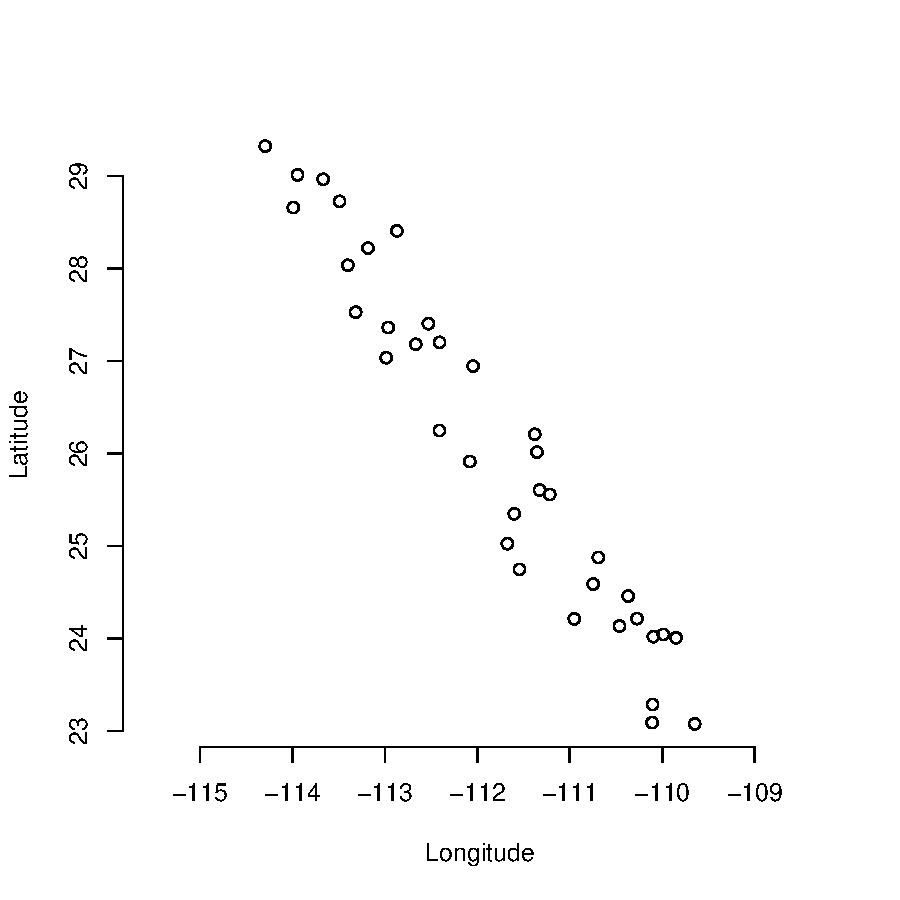
\includegraphics{gstudio-019}

Next, we can adjust the size of the symbol by diversity at any locus (below \texttt{LTRS} is used).  Here the \texttt{lapply} function is used to apply a function to the elements of the \texttt{baja.pops} list.  If you are not familiar with this function, you should look it up.  The resulting heterozyosity estimates are scaled and used as symbol size (via \texttt{cex}; Figure \ref{fig:araptus_he}).

\begin{Schunk}
\begin{Sinput}
> baja.pops <- partition( baja, "Pop" )
> pop.he <- lapply( baja.pops, function(x) he( Frequencies( x$LTRS ) ) )
> summary( unlist(pop.he) )
\end{Sinput}
\begin{Soutput}
   Min. 1st Qu.  Median    Mean 3rd Qu.    Max. 
 0.0000  0.0000  0.1800  0.2036  0.3457  0.4800 
\end{Soutput}
\begin{Sinput}
> plot(pop.coords, bty="n", xlab="Longitude", ylab="Latitude",asp=1,cex=2*unlist(pop.he)+1, main="Heterozygosity of LTRS")
\end{Sinput}
\end{Schunk}

\begin{figure}[bth]
	\centering
\begin{Schunk}
\begin{Sinput}
> baja.pops <- partition( baja, "Pop" )
> pop.he <- lapply( baja.pops, function(x) he( Frequencies( x$LTRS ) ) )
> summary( unlist(pop.he) )
\end{Sinput}
\begin{Soutput}
   Min. 1st Qu.  Median    Mean 3rd Qu.    Max. 
 0.0000  0.0000  0.1800  0.2036  0.3457  0.4800 
\end{Soutput}
\begin{Sinput}
> plot(pop.coords, bty="n", xlab="Longitude", ylab="Latitude",asp=1,cex=2*unlist(pop.he)+1, main="Heterozygosity of LTRS")
\end{Sinput}
\end{Schunk}
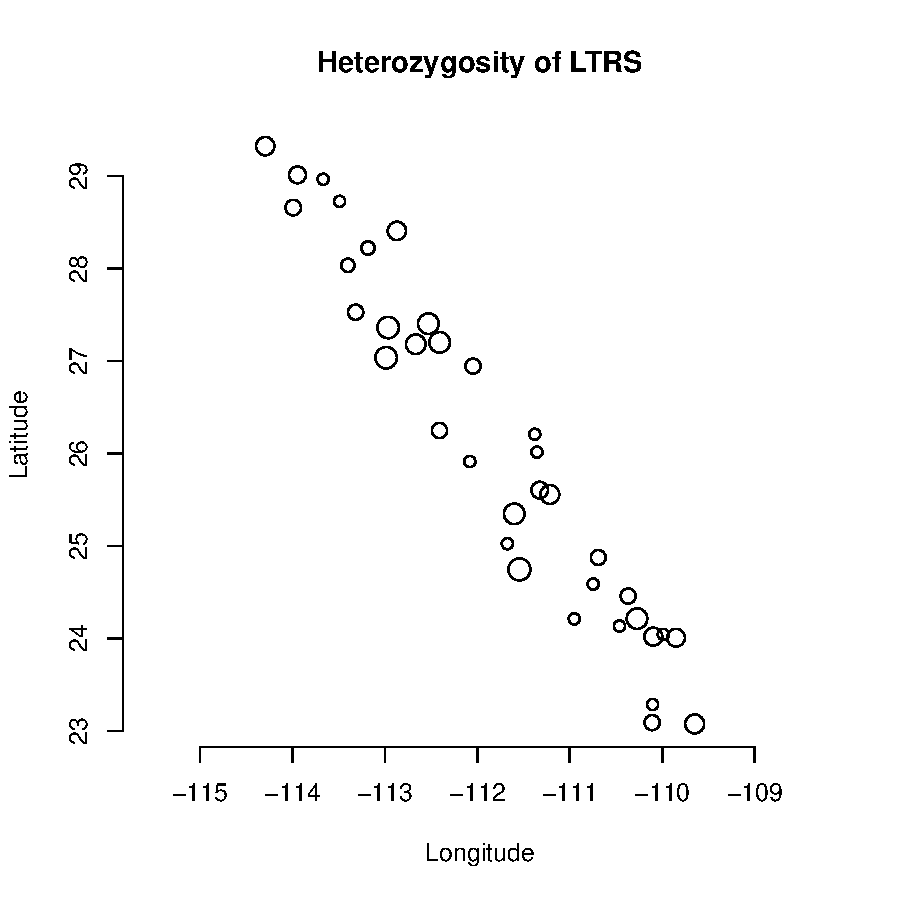
\includegraphics{gstudio-021}
	\caption{Heterozygosity of \emph{Araptus attenuatus} populations (depicted by symbol size) on the peninsula of Baja California.}
	\label{fig:araptus_he}
\end{figure}
\chapter{Genetic Diversity}

\section{Synopsis}

Genetic diversity is measure of within stratum variance and there are several methods available for the estimation of diversity.  In a general sense, we will be using measures of allelic richness from the Baja California data set, which can easily be found my examining the \texttt{Frequencies} of the loci.

\begin{Schunk}
\begin{Sinput}
> require(gstudio)
> data(araptus_attenuatus)
> baja <- araptus_attenuatus[araptus_attenuatus$Species != "CladeB",]
> freqs <- allele.frequencies(baja)
> freqs$LTRS
\end{Sinput}
\begin{Soutput}
Allele Frequencies:
  01 = 0.5519878 
  02 = 0.4480122 
\end{Soutput}
\begin{Sinput}
> freqs$MP20
\end{Sinput}
\begin{Soutput}
Allele Frequencies:
  07 = 0.2892308 
  05 = 0.2969231 
  15 = 0.001538462 
  08 = 0.02769231 
  06 = 0.08923077 
  04 = 0.009230769 
  18 = 0.1784615 
  19 = 0.009230769 
  17 = 0.04153846 
  10 = 0.01384615 
  11 = 0.04153846 
  16 = 0.001538462 
\end{Soutput}
\end{Schunk}

In this data set, the raw allelic diversity across all the samples range from 2 - 12 alleles.  However, using a base approach such as this falls short for several reasons:

\begin{enumerate}
	\item We are only looking at the number of alleles across the entire data set and there are many cases where it may be of interest to look at allelic diversity within substrata.  It is possible to use the \texttt{partition} function along with \texttt{allele.frequencies} to get to the number of alleles at partitions but the problem with that is:
	\item The raw number of alleles depends upon the number of individuals sampled.  It is not statistically sound to compare raw diversity of stratum with different numbers of individuals.  This is where \emph{rarefaction} comes in.
	\item The sole number of alleles present may not be as important as other measures of genetic diversity such as the diversity of non-rare alleles, or the average 'effective' number of alleles.
\end{enumerate}

To overcome both of these issues, the \texttt{genetic.diversity} function is used.

\subsection{Rarefaction}

Before we get into the nitty-gritty, the basic concept of rarefaction should be examined.  Rarefaction is a permutation technique that can be used to standardize samples based upon sample allocation and is an old friend to ecologists.  

For our purposes, we will consider rarefaction as a subsampling of alleles in strata standardized by the size of the smallest stratum.  So if we have one population with 10 individuals (20 alleles if the locus is diploid) and the rest of the populations have 50 individuals (100 alleles), a rarefied comparison of diversity should be based upon sampling of 20 alleles.

The function \texttt{genetic.diversity} takes random samples of the alleles within each population and recomputes the requested allelic diversity statistic.  While in many ecological studies, rarefaction is depicted as an accumulation curve (they are generally interested in sampling intensity), \texttt{genetic.diversity} only reports the distribution at the largest size where all strata are equal (e.g., the number of alleles present in the smallest population). 

\section{Allelic Diversity: $A$}

The parameter \emph{A} is solely a measure of the number of alleles at a locus.  If a population has a single individual with a single copy of allele $A$ and everyone else has allele $C$, $A=2$, which is the same case as if half the population was homozygous for $A$ and the remaining individuals were homozygous for $C$.  The function \texttt{genetic.diversity} returns an object that can be both printed and examined in plot fashion (by default it is a boxplot)

\begin{Schunk}
\begin{Sinput}
> A <- genetic.diversity(baja,stratum="Cluster",loci="MP20",mode="A")
> A
\end{Sinput}
\begin{Soutput}
Geneic Diversity:
  Estimator: A 
  Stratum: Cluster 
  Loci: { MP20 }
  Locus = MP20 
    CBP-C A = 5 ; Rarefaction A = 4.16716716716717 
    NBP-C A = 6 ; Rarefaction A = 3.51751751751752 
    SBP-C A = 2 ; Rarefaction A = 2 
    SCBP-A A = 4 ; Rarefaction A = 3.01601601601602 
\end{Soutput}
\begin{Sinput}
> plot(A)
\end{Sinput}
\end{Schunk}
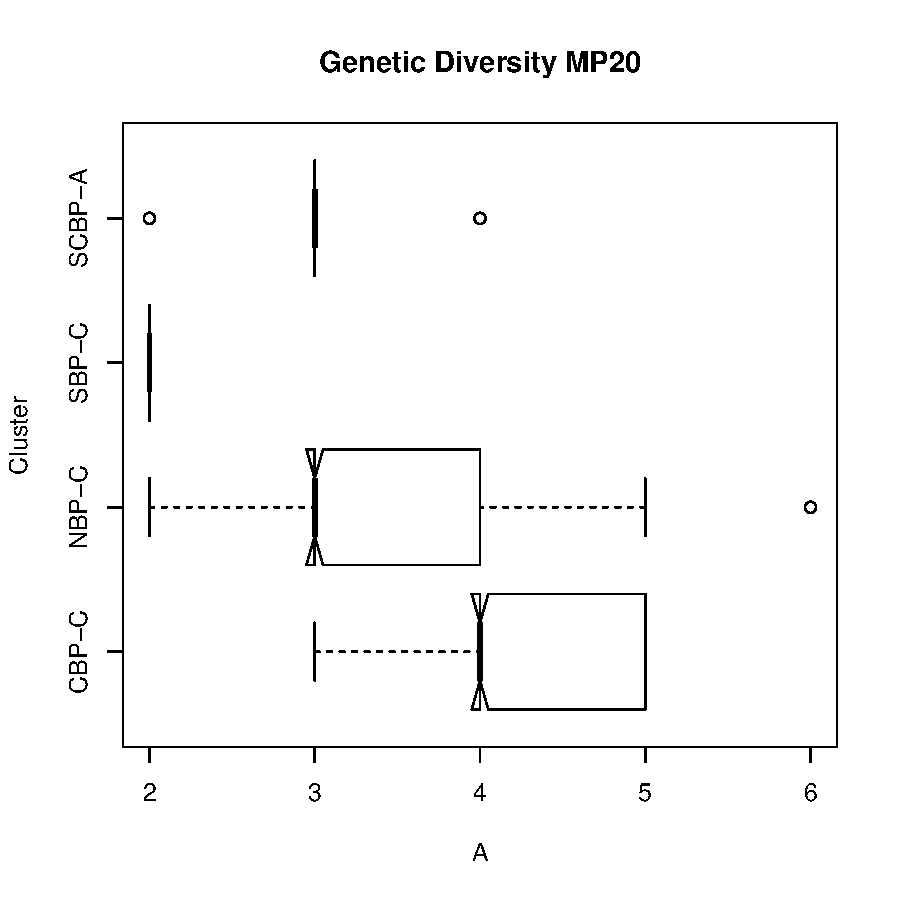
\includegraphics{gstudio-023}

The plot itself is a horizontal \texttt{boxplot}.  If you conduct the analysis with either the \texttt{loci} missing or as a list of loci, the results from each locus will be displayed in the terminal and the plotting will cycle through each locus requiring some input from the keyboard.  It is also possible to plot just a single locus by passing the locus name as a second parameter to the \texttt{plot} command.

\section{Allelic Diversity of Non-Rare Alleles: $A_{95}$}

The parameter $A_{95}$ ignores rare alleles by not counting those whose frequencies are below 95\% \emph{within} the stratum.  So alleles locally rare will not be counted and in general $A >= A_{95}$.

\begin{Schunk}
\begin{Sinput}
> A95 <- genetic.diversity(baja,stratum="Cluster",loci="MP20",mode="A95")
> A95
\end{Sinput}
\begin{Soutput}
Geneic Diversity:
  Estimator: A95 
  Stratum: Cluster 
  Loci: { MP20 }
  Locus = MP20 
    CBP-C A95 = 4 ; Rarefaction A95 = 3.65065065065065 
    NBP-C A95 = 2 ; Rarefaction A95 = 2.36436436436436 
    SBP-C A95 = 2 ; Rarefaction A95 = 2 
    SCBP-A A95 = 2 ; Rarefaction A95 = 2.45345345345345 
\end{Soutput}
\begin{Sinput}
> plot(A95)
\end{Sinput}
\end{Schunk}
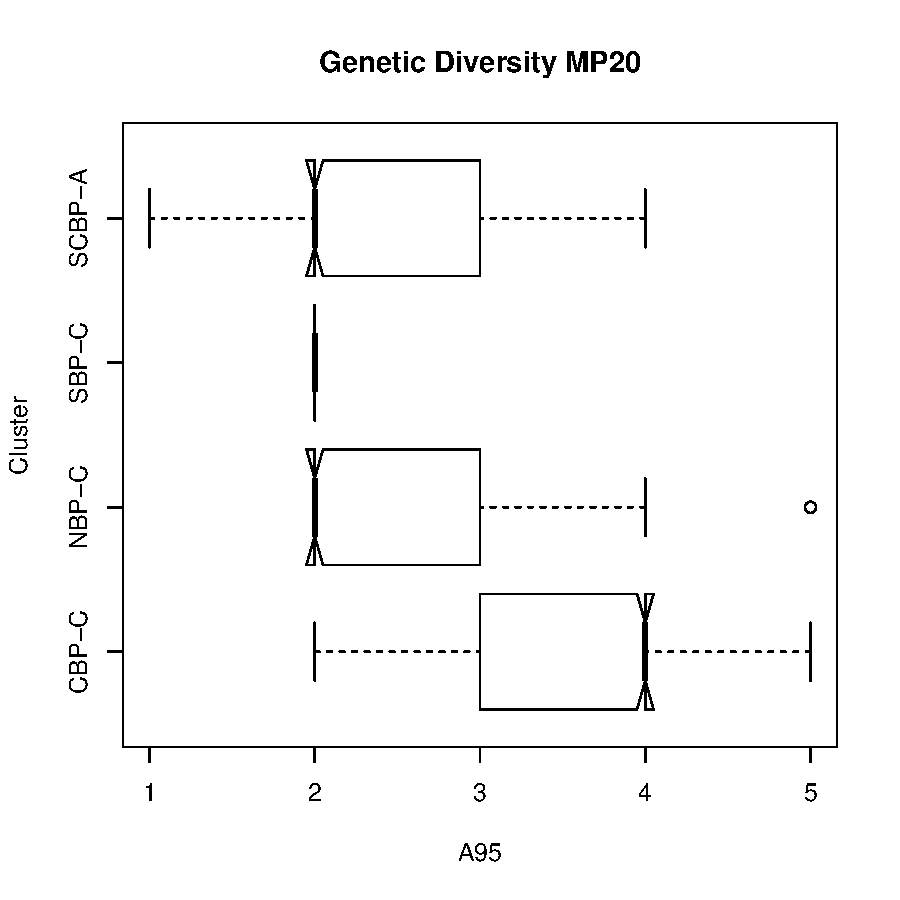
\includegraphics{gstudio-024}


\section{Effective Allelic Diversity: $A_e$}

The last diversity statistic is $A_e$, which is another frequency corrected allelic diversity statistic.  For a locus with $\ell$ alleles, each of which occurs at a frequency of $p_i$, the effective number of alleles is:

\begin{equation}
	A_e = \frac{1}{\sum_{i=1}^\ell p_i^2}
\end{equation}

And for the example data:

\begin{Schunk}
\begin{Sinput}
> Ae <- genetic.diversity(baja,stratum="Cluster",loci="MP20",mode="Ae")
> Ae
\end{Sinput}
\begin{Soutput}
Geneic Diversity:
  Estimator: Ae 
  Stratum: Cluster 
  Loci: { MP20 }
  Locus = MP20 
    CBP-C Ae = 2.93481610504455 ; Rarefaction Ae = 2.8455801976292 
    NBP-C Ae = 1.97536394176932 ; Rarefaction Ae = 1.95448118785927 
    SBP-C Ae = 1.6 ; Rarefaction Ae = 1.58736774866187 
    SCBP-A Ae = 1.58205596962453 ; Rarefaction Ae = 1.5793060658481 
\end{Soutput}
\begin{Sinput}
> plot(Ae)
\end{Sinput}
\end{Schunk}
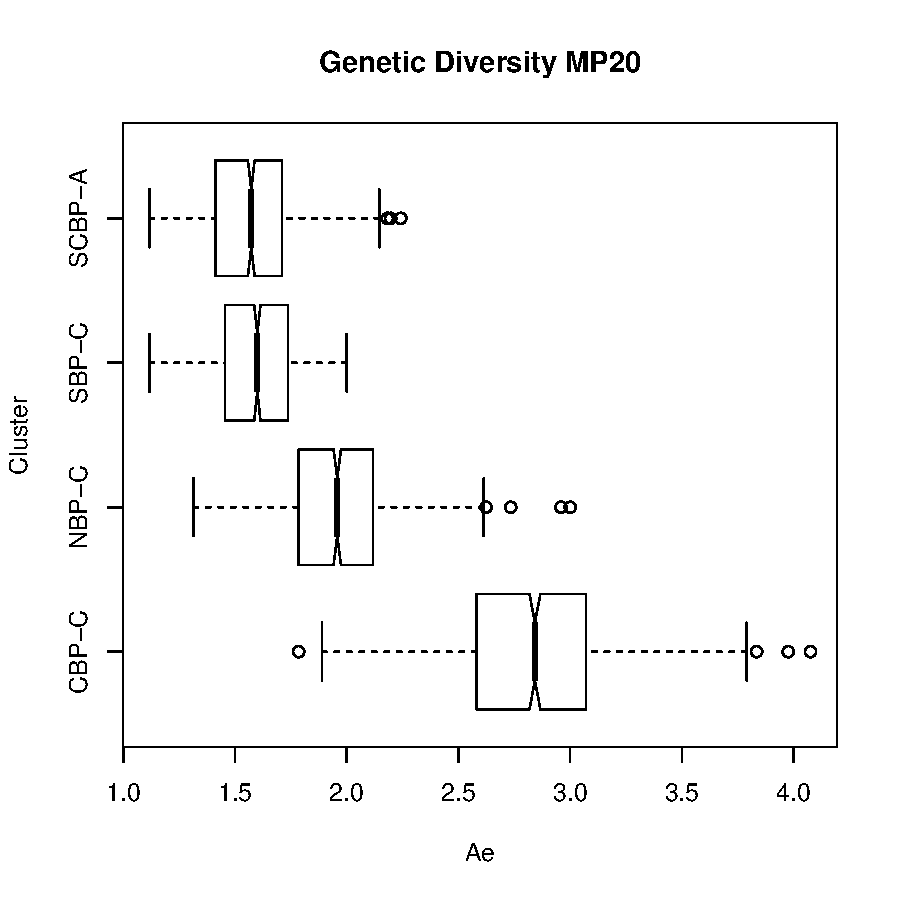
\includegraphics{gstudio-025}

One obvious difference in $A_e$ from the others is that it is not an integer value (both $A$ and $A95$ are integers) and as such can show a bit more granularity.

\chapter{Genetic Distance}

\section{Synopsis}

The analysis of genetic data is largely an analysis of distances; distances among frequencies, distances among centroids of populations, etc.

\section{Genetic Distances Among Individuals}

In these examples, the data from \emph{Araptus attenuatus} will be used again but this time we'll use the subset of individuals from "CladeB" (mainland populations).

\begin{Schunk}
\begin{Sinput}
> require(gstudio)
> data(araptus_attenuatus)
> sonora <- araptus_attenuatus[ araptus_attenuatus$Species=="CladeB" , ]
> summary(sonora)
\end{Sinput}
\begin{Soutput}
   Species    Cluster    Pop       Individual      Lat             Long       
 CladeB:36   SON-B:36   101: 9   101_10A: 1   Min.   :26.38   Min.   :-110.6  
                        102: 8   101_1A : 1   1st Qu.:26.64   1st Qu.:-109.6  
                        32 :19   101_2A : 1   Median :26.64   Median :-109.3  
                                 101_3A : 1   Mean   :26.90   Mean   :-109.6  
                                 101_4A : 1   3rd Qu.:26.95   3rd Qu.:-109.3  
                                 101_5A : 1   Max.   :27.91   Max.   :-109.1  
                                 (Other):30                                   
    LTRS       WNT         EN         EF        ZMP        AML        ATPS   
 01:01: 1   01:01:29   01:01: 7   01:01:23   01:01: 1   08:08: 1   02:02:28  
 01:02:17   01:03: 1   01:03: 2   01:02:11   02:02:19   08:11: 1   02:03: 1  
 02:02:18   NA   : 6   03:03:19   NA   : 2   NA   :16   08:12: 1   02:04: 2  
                       03:04: 6                         10:11: 1   02:09: 3  
                       04:04: 1                         11:11:12   04:04: 1  
                       NA   : 1                         12:12: 5   09:09: 1  
                                                        NA   :15             
      MP20   
 12:12  : 6  
 03:13  : 4  
 11:12  : 3  
 13:13  : 3  
 NA     : 3  
 02:10  : 2  
 (Other):15  
\end{Soutput}
\end{Schunk}

\subsection{Jaccard Distance}\index{Individual Distance!Jaccard}

Jaccard distance is a set-theoretic distance quantifying dissimilarity.  Assuming that loci are sets of alleles, the Jaccard dissimilarity between genotypes $A$ and $B$ is given by:

\begin{equation}
	J_\delta(A,B) = \frac{|A \bigcup B| - |A \bigcap B|}{|A \bigcup B|}
\end{equation}

Using the \texttt{LTRS} locus, we compute this distance as:

\begin{Schunk}
\begin{Sinput}
> d.jaccard <- genetic.distance(sonora,stratum="Pop",loci="EN",mode="Jaccard")
> dim(d.jaccard$LTRS)
\end{Sinput}
\begin{Soutput}
NULL
\end{Soutput}
\end{Schunk}

YOu can look at the elements of the LTRS matrix (it is 36x36 so I am not printing it out here).  With \texttt{mode="Jaccard"}, missing genotypes will result in \texttt{NA} rows and columns in the distance matrix.  It is no entirely clear how this metric can easily handle missing genotypes.

\subsection{Bray-Curtis Distance}\index{Individual Distance!Bray}

Bray-Curtis Distance (Bray \& Curtis 1957) has been primarily used to quantify differences in species composition.  It is defined as the total number of species that are unique to either of the two sites standardized by the number of species in both sites.  

\begin{equation}
	BC_\delta = \frac{S_i + S_j - 2S_{ij}}{S_i+S_j}
\end{equation}

where $S_x$ is the species count and $S_{ij}$ is the sum of minimum abundances.  Lately, this has seen considerable use within individual-based landscape genetic studies.  Missing genotypes are set to average allele frequencies, that is to say that every missing genotype is considered to have all the alleles present in the entire population, but with probability equal to their global frequencies.  Essentially, this removes the \texttt{NA} problem like in the \texttt{mode="Jaccard"} situation and does so by taking the non-missing genotype's genetic distance from the global genetic centroid (it's cosmic man!).  Here is the estimation using two loci.

\begin{Schunk}
\begin{Sinput}
> d.bray <- genetic.distance(sonora,stratum="Pop",loci=c("LTRS","EN"),mode="Bray")
> summary(d.bray)
\end{Sinput}
\begin{Soutput}
     Length Class  Mode   
LTRS 1296   -none- numeric
EN   1296   -none- numeric
\end{Soutput}
\end{Schunk}

\subsection{AMOVA Distance}\index{Individual Distance!AMOVA}

The final individual-based approach is based upon the Analysis of Molecular Variance (AMOVA) analysis.  A geometric interpretation of this genetic distance is given in Figure \ref{fig:amova_geometry} indicating distances among diploid genotypes.  

\begin{figure}[b]
	\centering
	\setlength{\unitlength}{2cm}
	\begin{picture}(3,2)
		\put(.8,.8){BB}
		\put(3,.8){CC}
		\put(1.88,2.02){AA}
		\put(1.2,1.5){AB}
		\put(2.6,1.5){AC}
		\put(1.88,.8){BC}
		\color{blue}
		\put(1.5,1.5){\line(1,-1){.5}}
		\put(2,2){\line(0,-1){1}}
		\color{black}
		\thicklines
		\put(1,1){\line(1,0){2}}
		\put(1,1){\line(1,1){1}}
		\put(3,1){\line(-1,1){1}}
		\color{red}
		\put(2,1.2){$\sqrt{3}$}
		\put(1.08,1.2){1}
		\put(1.64,1.75){1}
	\end{picture}
	\caption{Geometry of AMOVA distances.  The resulting squared distance is the square of the geometric distance.}
	\label{fig:amova_geometry}
\end{figure}

Algebraically, we can define an individual locus using a multivariate vector as an allele coding vector.  The \texttt{Locus} class has a method, \texttt{as.multivariate}, that does the translation.  The distance between the two alleles is defined as:

\begin{equation}
	\delta_{ij}^2 = 2(p_i-p_j)^2
\end{equation}

as shown below.


The amova distance is simply the vector distance between these two vectors as demonstrated below

\begin{Schunk}
\begin{Sinput}
> locAA <- Locus( c("A","A") )
> locBB <- Locus( c("B","B") )
> locAB <- Locus( c("A","B") )
> locBC <- Locus( c("B","C") )
> vAA <- as.vector( locAA, c("A","B","C") )
> vBB <- as.vector( locBB, c("A","B","C") )
> vAB <- as.vector( locAB, c("A","B","C") )
> vBC <- as.vector( locBC, c("A","B","C") )
> dist.AA.BB <- 2*( (vAA - vBB) %*% (vAA - vBB) )
> dist.AA.BB
\end{Sinput}
\begin{Soutput}
     [,1]
[1,]   16
\end{Soutput}
\begin{Sinput}
> dist.AA.AB <- 2*( (vAA - vAB) %*% (vAA - vAB) )
> dist.AA.AB
\end{Sinput}
\begin{Soutput}
     [,1]
[1,]    4
\end{Soutput}
\begin{Sinput}
> dist.AA.BC <- 2*( (vAA - vBC) %*% (vAA - vBC) )
> dist.AA.BC
\end{Sinput}
\begin{Soutput}
     [,1]
[1,]   12
\end{Soutput}
\end{Schunk}

While we will deal more with the AMOVA analysis in the section on Genetic Structure, the AMOVA genetic distance matrix can be estimated as follows, this time using \emph{all} the loci. This metric is additive across loci, so only a single distance matrix is returned.  The \texttt{list} key for the multilocus parameters is a list of the locus names, joined using a period.

\begin{Schunk}
\begin{Sinput}
> d.amova <- genetic.distance(sonora,stratum="Pop",mode="AMOVA",loci="EN")
> summary(d.amova)
\end{Sinput}
\begin{Soutput}
   Length Class  Mode   
EN 1296   -none- numeric
\end{Soutput}
\end{Schunk}


There are several other measures of individual-to-individual distance such as relatedness and coancestry.  These are not currently implemented in \texttt{R} but may become available in the near future.  That being said, it is probably something not too difficult for someone to extend these functions with their own code.

\subsection{Differences Between Distances}

These three distances are correlated, and here we can look at how close they are for this three allele locus in \emph{Euphorbia lomelii}.  They will be transformed from a \texttt{dist} matrix object into columns within a \texttt{data.frame} and then their relationship can be tested using \texttt{cor.test}.

\begin{Schunk}
\begin{Sinput}
> df <- data.frame( jaccard = d.jaccard$EN[lower.tri(d.jaccard$EN)],bray = d.bray$EN[lower.tri(d.bray$EN)], amova = d.amova$EN[lower.tri(d.amova$EN)])
> summary(df)
\end{Sinput}
\begin{Soutput}
    jaccard           bray            amova      
 Min.   :0.000   Min.   :0.0000   Min.   :0.000  
 1st Qu.:0.000   1st Qu.:0.0000   1st Qu.:0.000  
 Median :0.500   Median :0.5000   Median :1.000  
 Mean   :0.527   Mean   :0.5238   Mean   :1.568  
 3rd Qu.:1.000   3rd Qu.:1.0000   3rd Qu.:4.000  
 Max.   :1.000   Max.   :1.0000   Max.   :4.000  
\end{Soutput}
\begin{Sinput}
> cor(df)
\end{Sinput}
\begin{Soutput}
          jaccard      bray     amova
jaccard 1.0000000 0.9985311 0.8883334
bray    0.9985311 1.0000000 0.8919370
amova   0.8883334 0.8919370 1.0000000
\end{Soutput}
\begin{Sinput}
> pairs(df)
\end{Sinput}
\end{Schunk}

\begin{figure}[bth]
	\centering
\begin{Schunk}
\begin{Sinput}
> df <- data.frame( jaccard = d.jaccard$EN[lower.tri(d.jaccard$EN)],bray = d.bray$EN[lower.tri(d.bray$EN)], amova = d.amova$EN[lower.tri(d.amova$EN)])
> summary(df)
\end{Sinput}
\begin{Soutput}
    jaccard           bray            amova      
 Min.   :0.000   Min.   :0.0000   Min.   :0.000  
 1st Qu.:0.000   1st Qu.:0.0000   1st Qu.:0.000  
 Median :0.500   Median :0.5000   Median :1.000  
 Mean   :0.527   Mean   :0.5238   Mean   :1.568  
 3rd Qu.:1.000   3rd Qu.:1.0000   3rd Qu.:4.000  
 Max.   :1.000   Max.   :1.0000   Max.   :4.000  
\end{Soutput}
\begin{Sinput}
> cor(df)
\end{Sinput}
\begin{Soutput}
          jaccard      bray     amova
jaccard 1.0000000 0.9985311 0.8883334
bray    0.9985311 1.0000000 0.8919370
amova   0.8883334 0.8919370 1.0000000
\end{Soutput}
\begin{Sinput}
> pairs(df)
\end{Sinput}
\end{Schunk}
	\caption{Relationship among three individual genetic distance metrics estimated for individual \emph{Araptus attenuatus} individuals in Sonora \& Sinoloa, Mexico.}
	\label{fig:sonora_ind_dist}
\end{figure}




\clearpage

\section{Genetic Distance Among Strata}


Genetic distances can also be estimated among groups of individuals.  The same data will be used here but since there are only three populations, we'll be able to see the whole distance matrix. 


\subsection{Euclidean Distance}\index{Strata Distance!Euclidean}

Euclidean distance is the most straight-forward distance metric available as it is essentially straight-line distance based upon the allele frequencies in each population.  It is given by:

\[
	d_{eucl} = \sqrt{ \sum_{j=1}^L(p_{ij} - p_{kj})^2 }
\]


\begin{figure}[h!]
	\centering
	\setlength{\unitlength}{2cm}
	\begin{picture}(3,2)
		\put(0.08,0.08){0}
		\put(.8,0){$p_1$} 
		\put(0,.8){$p_2$}
		\put(0,1.5){1}
		\put(1.5,0){1}
		\thicklines
		\put(0.2,0.2){\vector(1,0){1.5}}
		\put(0.2,0.2){\vector(0,1){1.5}}
		\thinlines
		\put(0.6,1.39){\line(-1,0){0.4}}
		\put(0.6,1.39){\line(0,-1){1.19}}
		\put(1.39,0.6){\line(-1,0){1.19}}
		\put(1.39,0.6){\line(0,-1){0.4}}
		\color{red}
		\put(1.5,.6){X}
		\put(1.39,0.6){\circle*{.09}}
		\put(.6,1.5){Y}
		\put(0.6,1.39){\circle*{.09}}
		\color{black}
		\put(1.2,0){\footnotesize$p_{1,X}$}		
		\put(-.10,0.6){\footnotesize$p_{2,X}$}
		\put(-.10,1.39){\footnotesize$p_{2,Y}$}
		\put(0.4,0){\footnotesize$p_{1,Y}$}
		\thicklines
		\put(0.69,1.3){\vector(1,-1){.65}}
		\put(1.3,0.69){\vector(-1,1){.65}}	
	\end{picture}
	\caption{Geometry of euclidean distance based upon a two-allele locus denoted as frequencies $p_1$ \& $p_2$. }
	\label{fig:eucl_geometry}
\end{figure}

where $p_{ij}$ and $p_{kj}$ are the frequencies of the $j^{th}$ allele in both the $i^{th}$ and $j^{th}$ population.  In this and the following distance examples, I am going to take the resulting distance matrix among all pairs of populations and put them into a Neighbor joining tree (via the \texttt{nj} function from the \texttt{ape} package) as it may be easier to see differences in topologies rather than matrices.

It is perhaps easiest to think of Euclidean distance in x,y coordinate space (Figure \ref{fig:eucl_geometry}).  This distance can be estimated by \texttt{stratum.distance} using the optional parameter \texttt{method='eucl'} and it will return a \texttt{dist} matrix.

Once the matrix has been estimated, you can visualize it in many ways.  One of the most straight-forward approaches it to visualizing the relationships among rows and columns is to put it into a bifurcating tree.  
\begin{Schunk}
\begin{Sinput}
> d.eucl <- genetic.distance(sonora,stratum="Pop",loci="EN",mode="Euclidean")
> d.eucl
\end{Sinput}
\begin{Soutput}
$EN
          [,1]      [,2]      [,3]
[1,] 0.0000000 0.5611959 0.6908633
[2,] 0.5611959 0.0000000 0.2698923
[3,] 0.6908633 0.2698923 0.0000000
\end{Soutput}
\end{Schunk}






\subsection{Cavalli-Sforza Distance}\index{Strata Distance!Cavalli}

Another distance approach that is commonly used for microsatellite loci is Cavalli-Sforza distance, $D_C$ (Cavalli-Sforza and Edwards, 1967).  Here population allele frequencies are plot on the surface of a sphere (radius=1) using the square root of the allele frequencies.  

\[
	D_C = \frac{2}{\pi}\sqrt{(2-2cos\theta)}
\]

The genetic distance, $D_C$ is measured as the chord distance as indicated in Figure \ref{fig:cavalli_geometry}.  The resulting Neighbor joining tree from this distance is shown in Figure \ref{fig:cavalli_dist}

\begin{figure}[htbp]
	\centering
	\setlength{\unitlength}{2cm}
	\begin{picture}(3,2)
		\put(0.08,0.08){0}
		\put(0.7,0){$\sqrt{p_1}$} 
		\put(-0.2,.8){$\sqrt{p_2}$}
		\put(0,1.5){1}
		\put(1.5,0){1}
		\thicklines
		\put(0.2,0.2){\vector(1,0){1.5}}
		\put(0.2,0.2){\vector(0,1){1.5}}
		\put(0.0,0.0){\arc(1.50,0.20){75}}
		\color{red}
		\put(1.5,.6){X}
		\put(1.39,0.6){\circle*{.09}}
		\put(.6,1.5){Y}
		\put(0.6,1.39){\circle*{.09}}
		\color{black}
		\thicklines
		\put(0.69,1.3){\vector(1,-1){.65}}
		\put(1.3,0.69){\vector(-1,1){.65}}
	\end{picture}
	\caption{Geometry of Cavalli-Sforza distance.  Population allele frequencies at two loci are plot at$\sqrt{p_1}$ and $\sqrt{p_2}$ and $D_C$ is the chord between the populations.}
	\label{fig:cavalli_dist}
\end{figure}


\begin{Schunk}
\begin{Sinput}
> d.cavalli <- genetic.distance(sonora,"Pop","EN","Cavalli")
> d.cavalli
\end{Sinput}
\begin{Soutput}
$EN
          [,1]      [,2]      [,3]
[1,] 0.0000000 0.4131725 0.7554523
[2,] 0.4131725 0.0000000 0.5155875
[3,] 0.7554523 0.5155875 0.0000000
\end{Soutput}
\end{Schunk}




\subsection{Nei's Genetic Distance}\index{Strata Distance!Nei}

Nei's genetic distance is based upon mutation drift equilibrium therefore you should be reasonably comfortable with the notion that your populations have been separated a sufficient period of time such that drift and mutation may have played a significant role in their structure.

The formula for Nei's distance that is used here is: 

\[
	D_{Nei} = -ln\left(\frac{(2N-1)\sum_{i=1}^L\sum_{j=1}^\ell p_{ij,x}p_{ij,y}}{\sqrt{\sum_{i=1}^L(2N\sum_{j=1}^\ell p_{ij,x}-1)(2N\sum_{j=1}^\ell p_{ij,y}-1)}} \right)
\]

where the summation $L$ is across loci and $\ell$ is across alleles at each locus in population $x$ and $y$.



\begin{Schunk}
\begin{Sinput}
> d.nei <- genetic.distance(sonora,"Pop","EN","Nei")
> d.nei
\end{Sinput}
\begin{Soutput}
$EN
          [,1]     [,2]      [,3]
[1,] 0.0000000 1.200027 0.5848357
[2,] 1.2000270 0.000000 2.8444285
[3,] 0.5848357 2.844428       Inf
\end{Soutput}
\end{Schunk}


 


\subsection{Conditional Genetic Distance}\index{Strata Distance!cGD}

Conditional genetic distance ($cGD$, Dyer et al. 2010) is a graph-theoretic genetic distance derived from Population Graphs (Dyer and Nason 2004).  In some cases it has been shown to be more sensitive to landscape features and heterogeneity in dispersal than structure statistics and other distance metrics (see Dyer et al. 2010).

\begin{Schunk}
\begin{Sinput}
> d.cgd <- genetic.distance(sonora,"Pop","EN","cGD")
\end{Sinput}
\begin{Soutput}
tranforming data... done
Rotating mv genos and partitioning...  done
Estimating conditional genetic covariance... done
Making graph... done
\end{Soutput}
\begin{Sinput}
> d.cgd
\end{Sinput}
\begin{Soutput}
$EN
         [,1]     [,2]     [,3]
[1,] 0.000000 4.154197 2.477791
[2,] 4.154197 0.000000 2.010668
[3,] 2.477791 2.010668 0.000000
\end{Soutput}
\end{Schunk}




\section{Isolation-By-Distance}


Under models with restrictions in gene flow, there is an expectation that genetic distance should increase with physical separation.  Using populations found along the Baja Peninsula, it is pretty easy to see which one of these among-strata distance approaches provides a better fit to the data.

\begin{Schunk}
\begin{Sinput}
> baja <- araptus_attenuatus[araptus_attenuatus$Species != "CladeB", ]
> euc <- genetic.distance(baja,"Pop","EN","Euclidean")$EN
> cav <- genetic.distance(baja,"Pop","EN","Cavalli")$EN
> nei <- genetic.distance(baja,"Pop","EN","Nei")$EN
> cgd <- genetic.distance(sonora,"Pop","EN","cGD")$EN
\end{Sinput}
\begin{Soutput}
tranforming data... done
Rotating mv genos and partitioning...  done
Estimating conditional genetic covariance... done
Making graph... done
\end{Soutput}
\begin{Sinput}
> phys <- stratum.distance(baja,"Pop",lat="Lat",lon="Long")
> df <- data.frame(Euclidean=euc[lower.tri(euc)], Cavalli=cav[lower.tri(cav)], Nei=nei[lower.tri(nei)], cGD=cgd[lower.tri(cgd)], Physical.Dist=phys[lower.tri(phys)] )
> pairs( df )
> cor(df)
\end{Sinput}
\begin{Soutput}
               Euclidean    Cavalli Nei        cGD Physical.Dist
Euclidean     1.00000000 0.94146219 NaN 0.09490699    0.29356944
Cavalli       0.94146219 1.00000000 NaN 0.08888958    0.27044432
Nei                  NaN        NaN   1        NaN           NaN
cGD           0.09490699 0.08888958 NaN 1.00000000    0.02110107
Physical.Dist 0.29356944 0.27044432 NaN 0.02110107    1.00000000
\end{Soutput}
\end{Schunk}


\begin{figure}[bth]
	\centering
\begin{Schunk}
\begin{Sinput}
> baja <- araptus_attenuatus[araptus_attenuatus$Species != "CladeB", ]
> euc <- genetic.distance(baja,"Pop","EN","Euclidean")$EN
> cav <- genetic.distance(baja,"Pop","EN","Cavalli")$EN
> nei <- genetic.distance(baja,"Pop","EN","Nei")$EN
> cgd <- genetic.distance(sonora,"Pop","EN","cGD")$EN
\end{Sinput}
\begin{Soutput}
tranforming data... done
Rotating mv genos and partitioning...  done
Estimating conditional genetic covariance... done
Making graph... done
\end{Soutput}
\begin{Sinput}
> phys <- stratum.distance(baja,"Pop",lat="Lat",lon="Long")
> df <- data.frame(Euclidean=euc[lower.tri(euc)], Cavalli=cav[lower.tri(cav)], Nei=nei[lower.tri(nei)], cGD=cgd[lower.tri(cgd)], Physical.Dist=phys[lower.tri(phys)] )
> pairs( df )
> cor(df)
\end{Sinput}
\begin{Soutput}
               Euclidean    Cavalli Nei        cGD Physical.Dist
Euclidean     1.00000000 0.94146219 NaN 0.09490699    0.29356944
Cavalli       0.94146219 1.00000000 NaN 0.08888958    0.27044432
Nei                  NaN        NaN   1        NaN           NaN
cGD           0.09490699 0.08888958 NaN 1.00000000    0.02110107
Physical.Dist 0.29356944 0.27044432 NaN 0.02110107    1.00000000
\end{Soutput}
\end{Schunk}
	\caption{Relationship among strata genetic distance metrics estimated for \emph{Araptus attenuatus} sites in Baja California along with physical distance.}
	\label{fig:sonora_strata_dist}
\end{figure}


\chapter{Genetic Structure}


\section{Synopsis}

Estimation of genetic structure is a fundamental process in population genetic analyses.  Broadly defined, structure can be defined as the non-random association of genotypes and alleles in populations due to evolutionary processes such as gene flow, drift, selection, and inbreeding.  For this, the \emph{Araptus attenuatus} data set and will be used again.

\begin{Schunk}
\begin{Sinput}
> require(gstudio)
> data(araptus_attenuatus)
> baja <- araptus_attenuatus[araptus_attenuatus$Species != "CladeB",]
\end{Sinput}
\end{Schunk}

\section{Genotype Frequencies}

The manner by which alleles are arranged into genotypes tells us a lot about the history of a species.  The structure statistic that are presented below all rely upon estimation of genotype frequencies so a brief digression to talk about genotype frequencies is in order.

Under a model of random mating, a locus with $\ell$ alleles whose frequencies are denoted by $p_1, p_2, \ldots, p_\ell$, homozygotes for the $i^{th}$ allele are expected to occur at a frequency of $p_i^2$ and $ij$-heterozygotes are expected at $2p_ip_j$.


The expected frequencies are estimated from the allele frequencies assuming Hardy-Weinberg Equilibrium.  If you were only interested in the proportion of heterozygotes, you can use the \texttt{ho} and \texttt{he} functions.   

\begin{Schunk}
\begin{Sinput}
> freq.ltrs <- allele.frequencies(baja, "LTRS")
> he(freq.ltrs$LTRS)*length(baja$LTRS)
\end{Sinput}
\begin{Soutput}
      he 
161.7324 
\end{Soutput}
\begin{Sinput}
> ho(freq.ltrs$LTRS)*length(baja$LTRS)
\end{Sinput}
\begin{Soutput}
ho 
69 
\end{Soutput}
\end{Schunk}

However, at times, it is of interest to look at all genotypes.  If you use the \texttt{as.character} method for \texttt{Locus} objects, you can easily tabulate the counts of each genotypic state\footnote{This function does take into consideration the non-sorting nature of the \texttt{Locus} object so that a \texttt{3:4} locus and a \texttt{4:3} locus will be counted as the same heterozygote.}. 

\begin{Schunk}
\begin{Sinput}
> obs <- genotype.counts( araptus_attenuatus, "LTRS")
> obs
\end{Sinput}
\begin{Soutput}
01:01 01:02 02:02 
  147    86   130 
\end{Soutput}
\begin{Sinput}
> obs/sum(obs)
\end{Sinput}
\begin{Soutput}
    01:01     01:02     02:02 
0.4049587 0.2369146 0.3581267 
\end{Soutput}
\end{Schunk}

Below they are denoted as a matrix, the values on the diagonal of \texttt{exp} are the expected number of homozygotes and off-diagonal estimates are the expected frequency of heterozygotes.

\begin{Schunk}
\begin{Sinput}
> p <- get.frequencies( freq.ltrs$LTRS )
> p
\end{Sinput}
\begin{Soutput}
       01        02 
0.5519878 0.4480122 
\end{Soutput}
\begin{Sinput}
> exp.freq <- p %*% t(p) 
> row.names(exp.freq) <- colnames(exp.freq)
> exp <- exp.freq * length(baja$LTRS)
> exp
\end{Sinput}
\begin{Soutput}
         01       02
01 99.63379 80.86621
02 80.86621 65.63379
\end{Soutput}
\end{Schunk}

As you can see there are fewer heterozygotes than expected ($N_{hets;\;exp}=$ 162, $N_{hets;\;obs}=$86). 

\section{Hardy-Weinberg Equilibrium}

While the \texttt{gstudio} package provides the basic units for population genetic analyses, there are already some very good packages that conduct analyses like testing for Hardy-Weinberg Equilbrium\footnote{There are many other functional packages on cran.r-project.org and you should always make sure someone hasn't already solved a problem for you before you try to code up a solution.}.

\begin{Schunk}
\begin{Sinput}
> require(HardyWeinberg)
> ltrs.genoytpes <- genotype.counts( araptus_attenuatus, "LTRS")
> HWChisq(ltrs.genoytpes,verbose=T)
\end{Sinput}
\begin{Soutput}
Chi-square test with continuity correction for Hardy-Weinberg equilibrium
Chi2 =  98.52808 p-value =  0 D =  -47.55096 
$chisq
[1] 98.52808

$pval
[1] 0

$D
    01:02 
-47.55096 

$p
   01:01 
0.523416 
\end{Soutput}
\end{Schunk}


\section{Structure Parameters}

Population structure parameters are fundamental tools for population genetics and have been perhaps, the most poorly understood and misused as well.  At the end of this section, some examples of the differences between the parameters is given.

These structure parameters are estimated using the function \texttt{genetic.structure} and requires a \texttt{Population} object, a \texttt{stratum}, the \texttt{loci} you want to estimate parameters from, and a \texttt{mode} (the parameter you want).  If you leave off the \texttt{loci} parameter, all loci will be used.  There is also an optional parameter, \texttt{num.perm} that is used to test significance.  

Finally, of note here is that all these parameters use a sample-size corrected estimates of heterozygosity.

\begin{align*}
	\hat{H}_S & = \frac{2\mu}{2\mu-1}H_S \\
	\hat{H}_T & =  H_T + \frac{\hat{H}_S}{2k\mu} 
\end{align*}

Where $\mu$ is the harmonic mean strata size and k is the number of stratum.  As you can see as $\mu$ gets larger $\hat{H}_S \to H_S$, which translates to "if you have more samples, you can get a better estimate of the average heterozygosity" and as $k$ get larger, $\hat{H}_T \to H_T$ which says the same thing about the number of populations.  The take-home here is that you need many samples from many places.


\subsection{The $G_{ST}$ Parameter}

The parameter $G_{ST}$ is an estimate of the reduction in heterozygosity due to individuals being in different populations.  It is functionally equivalent to $F_{ST}$ from Wright and as he points out, it is not a measure of differentiation in the way that we think of differentiation.  Rather it is a measure of the extent to which populations have gone to fixation.  It is estimated as: 

\[
G_{ST} = 1 - \frac{\hat{H}_S}{\hat{H}_T}
\]

where $H_S$ is the average expected heterozygosity at each stratum $[1-\sum_{i=1}^\ell p_i^2]/K$ and $H_T$ is the expected heterozygosity across the entire dataset.  

For the \emph{EN} locus in the Baja California dataset, $G_{ST}$ is estimated by:

\begin{Schunk}
\begin{Sinput}
> gst.baja <- genetic.structure(baja,stratum="Pop",loci="EN",mode="Gst",num.perm=999)
> print(gst.baja)
\end{Sinput}
\begin{Soutput}
Geneic Structure Analysis:
  Estimator: Gst 
  Stratum: Pop 
  Loci: { EN }
   - EN ;  Gst = 0.345786963051191 ; P = 0.001 
\end{Soutput}
\end{Schunk}

\subsection{The $G_{ST}^\prime$ Parameter}

The parameter $G_{ST}^\prime$ was introduced by Hedrick (20XX) in response to the observation that the parameter $G_{ST}$ is not insensitive to the number of alleles at a locus.  Fixing this is done by standardizing the estimate of $G_{ST}$ by the maximal is can be given the number of alleles present, essential a restandardization to the [0,1] range.  This is done by:

\[
G_{ST}^\prime = \frac{G_{ST}(k-1+\mu)}{(k-1)(1-\hat{H}_S)}
\]

For the same locus, we get a larger

\begin{Schunk}
\begin{Sinput}
> gst.prime.baja <- genetic.structure(baja,stratum="Pop","EN",mode="Gst.prime",num.perm=999)
> print(gst.prime.baja)
\end{Sinput}
\begin{Soutput}
Geneic Structure Analysis:
  Estimator: Gst.prime 
  Stratum: Pop 
  Loci: { EN }
   - EN ;  Gst.prime = 0.459618108931204 ; P = 0.001 
\end{Soutput}
\end{Schunk}



\subsection{The $D_{EST}$ Parameter}

It has been pointed out that even with the corrections for large numbers of alleles, $G_{ST}^\prime$ may not be acting like a statistic of "differentiation" in the way that we think of differentiation.  For example consider the following code where I make three populations, the first one fixed for the "1" allele and the next fixed for the "2" (sure this is an extreme point, but Wright originally made it and it should be repeated).

\begin{Schunk}
\begin{Sinput}
> locus1 <- list()
> for(i in 1:50)
+ 	locus1[i] <- Locus( c(1,1) )
> for(i in 51:150)
+ 	locus1[i] <- Locus( c(2,2) )
> strata <- c(rep("Pop-A",50), rep("Pop-B",50), rep("Pop-C",50) )
> pop <- Population(strata=strata, loci=locus1)
> summary(pop)
\end{Sinput}
\begin{Soutput}
    strata           loci    
 Length:150         1:1: 50  
 Class :character   2:2:100  
 Mode  :character            
\end{Soutput}
\end{Schunk}

When we estimate either $G_{ST}$ or $G_{ST}$ on these data we get:

\begin{Schunk}
\begin{Sinput}
> genetic.structure(pop,"strata","loci",mode="Gst")
\end{Sinput}
\begin{Soutput}
Geneic Structure Analysis:
  Estimator: Gst 
  Stratum: strata 
  Loci: { loci }
   - loci ;  Gst = 1 
\end{Soutput}
\begin{Sinput}
> genetic.structure(pop,"strata","loci",mode="Gst.prime")
\end{Sinput}
\begin{Soutput}
Geneic Structure Analysis:
  Estimator: Gst.prime 
  Stratum: strata 
  Loci: { loci }
   - loci ;  Gst.prime = 1 
\end{Soutput}
\end{Schunk}

Now, intuitively, if it were just "Pop-A" and "Pop-B" then this would make sense but look at the differences between "Pop-B" and "Pop-C", this should be $G_{ST} = G_{ST}^\prime = 0$!  In fact, if you had only one population fixed for the "1" allele and a thousand populations fixed for the other, these parameters would still equal unity.  This is because, as Wright originally pointed out, these population parameters are not meant to measure differentiation but fixation.  The parameter $D_{est}$ was introduced by Joost (20XX) to address this issue (n.b., Gregorious proposed this back in the 80's but was not taken serious about it then, perhaps Joost can have better luck).

The parameter is defined as:

\[
D_{est} = \frac{k-1}{k} \frac{\hat{H}_T - \hat{H}_S}{1-\hat{H}_S}
\]

For the contrived data set, it gives:

\begin{Schunk}
\begin{Sinput}
> genetic.structure(pop,"strata","loci","Dest")
\end{Sinput}
\begin{Soutput}
Geneic Structure Analysis:
  Estimator: Dest 
  Stratum: strata 
  Loci: { loci }
   - loci ;  Dest = 0.296296296296296 
\end{Soutput}
\end{Schunk}

Which is what would be expected, roughly a third, if we have two populations that are identical and one that is differentiated from the rest.  I recommend looking at the several papers that go over these issues for more clarity.

For completeness, the results of the Baja California data set, under $D_{est}$ are:

\begin{Schunk}
\begin{Sinput}
> Dest.baja <- genetic.structure(baja,stratum="Pop","EN",mode="Dest",num.perm=999)
> print(Dest.baja)
\end{Sinput}
\begin{Soutput}
Geneic Structure Analysis:
  Estimator: Dest 
  Stratum: Pop 
  Loci: { EN }
   - EN ;  Dest = 0.164464814867075 ; P = 0.001 
\end{Soutput}
\end{Schunk}

\section{Pairwise Structure}

The \texttt{genetic.structure} function can also be used to estimate pairwise estimates of each parameter using the optional \texttt{pairwise} flag.  

\begin{Schunk}
\begin{Sinput}
> sonora <- araptus_attenuatus[araptus_attenuatus$Species=="CladeB",]
> genetic.structure(sonora,"Pop",loci="EN",mode="Gst.prime", pairwise=TRUE)
\end{Sinput}
\begin{Soutput}
          101        32       102
101 0.0000000 0.4136727 0.3661894
32  0.4136727 0.0000000 0.1245850
102 0.3661894 0.1245850 0.0000000
\end{Soutput}
\end{Schunk}
%
%  GStudio Documentation: DataImport
%
%  Created by dyer on 2011-07-20.



\chapter{Parent Offspring Data}

\section{Synopsis}

There are several cases where you have data that consists of both adults and offspring.  With these kinds of data, there are some interesting kinds of analyses available for examining structure and diversity.  The functionality that \texttt{gstudio} provides focuses on translations of offspring data into common formats that can be analyzed using regular routines.


\section{Getting Data}

The use of GoogleDocs as a repository for your data is not unique to parent-offspring data and is used here to demonstrate how to utilize this options.  There is a more detailed discussion of how to set up your GoogleSpreadsheets so that you can access them in the \texttt{DataImport} vignette.  In what follows, I will use the \emph{Cornus florida} data.  I split URL (see Data Import) because it was so long it trailed off the page...  

\begin{Schunk}
\begin{Sinput}
> require(gstudio)
> data(cornus_florida)
> cornus <- cornus_florida
\end{Sinput}
\end{Schunk}

The structure of adult/offspring data is just like any other kind of data and can consist of covariates such as physical location, size, etc. along with strata and loci.  The distinction is that there must be \emph{at least} two strata columns:
\begin{description}
	\item[Individual ID] There should a column in the dataset that has identification number or names that are unique to adults.  Every adult \emph{must} have a unique identification numver.
	\item[Offspring ID] To differentiate offspring from adults, the Offspring ID column should have the maternal individual (or paternal if you like) equal to 0.  Offspring from this individual have non-zero values for the Offspring ID column.  Offspring do not need to all have unique Offspring ID designations, just unique ones within the set of offspring with the same Individual ID.  
\end{description}

Here is an example to show the distinctions. 

\begin{Schunk}
\begin{Sinput}
> family <- offspring.array(cornus,474)
> family
\end{Sinput}
\begin{Soutput}
$mom
  IndID OffID    X    Y      G8     H18      N5     N10      O5
1   474     0 1545 2234 156:164 104:112 126:126 198:200 185:193

$offspring
   IndID OffID    X    Y      G8     H18      N5     N10      O5
1    474     1 1545 2234 164:168 104:112 126:126 198:202 185:195
2    474     2 1545 2234 156:156 102:112 126:126 198:198 179:185
3    474     3 1545 2234 162:164 112:114 124:126 192:198 185:193
4    474     4 1545 2234 164:188 110:112 126:126 194:198 185:193
5    474     5 1545 2234 156:158 112:112 126:128 192:198 185:193
6    474     6 1545 2234 164:180 108:112 126:126 188:198 177:193
7    474     7 1545 2234 164:188 110:112 126:126 190:198 177:185
8    474     8 1545 2234 164:168 104:112 126:126 200:202 193:193
9    474     9 1545 2234 156:164 112:112 126:126 190:198 185:193
10   474    10 1545 2234 164:188 110:112 126:126 190:198 177:185
11   474    11 1545 2234 164:168 110:112 126:126 188:200 181:185
12   474    12 1545 2234 164:180 112:112 126:126 190:198 179:193
13   474    13 1545 2234 164:164 112:114 126:126 188:198 181:185
14   474    14 1545 2234 156:180 112:118 126:126 188:200 185:193
15   474    15 1545 2234 156:180 112:114 126:126 190:200 179:185
16   474    16 1545 2234 156:168 104:112 126:126 192:198 193:193
17   474    17 1545 2234 164:164 112:112 126:126 198:200 193:193
18   474    18 1545 2234 156:164 104:114 126:126 198:202 181:193
19   474    19 1545 2234 164:164 112:112 126:128 198:200 185:193
20   474    20 1545 2234 164:168 112:112 126:126 192:198 193:193
\end{Soutput}
\end{Schunk}

Notice that all the offspring from mom '474' have the same IndID and she is differentiated from the offspring by having 'OffID=0'.  In fact, all the adults in the dataset can be found as:

\begin{Schunk}
\begin{Sinput}
> adults <- cornus[cornus$OffID==0,]
> adults
\end{Sinput}
\begin{Soutput}
   IndID OffID    X    Y      G8     H18      N5     N10      O5
1    226     0 1392 3534 162:180 114:114 124:126 192:192 185:195
2    232     0 1656 3414 158:180 112:112 124:126 184:192 185:185
3    234     0 1718 3330 158:180  112:96 128:128 184:192 185:185
4    300     0 1175 3114 180:188 112:116 126:126 198:200 191:195
5    305     0 1529 3237 154:170 122:124 124:126 188:192 181:195
6    432     0 1336 2748 164:180 114:116 124:126 198:202 185:193
7    433     0 1337 2749 180:188 112:114 126:126 198:202 179:193
8    468     0 1588 2233 164:164 110:116 124:124 198:202 181:193
9    474     0 1545 2234 156:164 104:112 126:126 198:200 185:193
10   484     0 1514 2302 160:168 112:116 126:126 192:192 193:193
11   487     0 1517 2305 164:176 110:112 126:126 192:202 179:181
12   489     0 1519 2307 160:164 104:112 126:126 192:202 179:181
13   490     0 1520 2308 164:176 112:112 128:128 192:202 179:181
14   493     0 1523 2311 168:168 104:112 124:126 192:202 193:195
15   512     0 1174 2279 156:174 108:114 126:126 200:202 179:195
16   513     0 1239 2276 156:180 102:114 126:126 190:198 179:179
17   516     0 1299 2135 156:180 102:114 124:126 190:198 179:179
18   519     0 1357 2148 156:180 104:114 126:126 182:188 181:181
19   520     0 1412 2041 164:172 114:124 126:126 188:198 195:195
20   521     0 1511 1949 160:164 112:112 128:128 198:200 185:193
21   590     0 1880 1040 164:168 112:118 124:126 192:198 177:193
22   607     0 2286 2888 154:164 114:114 126:126 188:202 181:181
\end{Soutput}
\end{Schunk}


\section{Pollen Pools}

Since my research is primarily focused on the analysis of plant populations and mother/offspring combinations provide information about pollen donors, naturally these kinds of analyses will be the first kind to have functionality.

\subsection{Minus Mom}

If you have the collection of offspring and a mother, you can estimate pollen pool allele frequencies as by subtracting the maternal contribution to each genotype and then estimating the allele frequencies of the paternal components (this could be reversed if you have father/offspring data and need to estimate maternal genotype frequencies just as easily).

\begin{Schunk}
\begin{Sinput}
> offs <- minus.mom( cornus )
> offs
\end{Sinput}
\begin{Soutput}
   IndID OffID    X    Y      G8     H18  N5     N10      O5
1    468     1 1588 2233     156     112 126     200     185
2    468     2 1588 2233     180     112 126 198:202     193
3    468     3 1588 2233     188     114 126     198     179
4    468     4 1588 2233     180     112 126     192     185
5    468     5 1588 2233     154     104 126     202     195
6    468     6 1588 2233     154     104 124     188     193
7    468     7 1588 2233     162     114 124     192     185
8    468     8 1588 2233     180     114 126     192     195
9    468     9 1588 2233     180     114 126     202     193
10   468    10 1588 2233     182     114 124     184     195
11   468    11 1588 2233     158     112 128     192     185
12   468    12 1588 2233     158     112 128     192     185
13   468    13 1588 2233     164     108 126     188     191
14   468    14 1588 2233     182     108 126 198:202 181:193
15   468    15 1588 2233     180     112 126 198:202 181:193
16   468    16 1588 2233     164     102 126     198 181:193
17   468    17 1588 2233     164     104 126     188     193
18   468    18 1588 2233     182     108 126 198:202 181:193
19   468    19 1588 2233     182     104 126     202 181:193
20   468    20 1588 2233     182     110 126 198:202     179
21   474     1 1545 2234     168 104:112 126     202     195
22   474     2 1545 2234     156     102 126     198     179
23   474     3 1545 2234     162     114 124     192 185:193
24   474     4 1545 2234     188     110 126     194 185:193
25   474     5 1545 2234     158     112 128     192 185:193
26   474     6 1545 2234     180     108 126     188     177
27   474     7 1545 2234     188     110 126     190     177
28   474     8 1545 2234     168 104:112 126     202     193
29   474     9 1545 2234 156:164     112 126     190 185:193
30   474    10 1545 2234     188     110 126     190     177
31   474    11 1545 2234     168     110 126     188     181
32   474    12 1545 2234     180     112 126     190     179
33   474    13 1545 2234     164     114 126     188     181
34   474    14 1545 2234     180     118 126     188 185:193
35   474    15 1545 2234     180     114 126     190     179
36   474    16 1545 2234     168 104:112 126     192     193
37   474    17 1545 2234     164     112 126 198:200     193
38   474    18 1545 2234 156:164     114 126     202     181
39   474    19 1545 2234     164     112 128 198:200 185:193
40   474    20 1545 2234     168     112 126     192     193
\end{Soutput}
\begin{Sinput}
> freqs.G8 <- Frequencies(offs$G8)
> freqs.G8
\end{Sinput}
\begin{Soutput}
Allele Frequencies:
  156 = 0.0952381 
  180 = 0.2142857 
  188 = 0.0952381 
  154 = 0.04761905 
  162 = 0.04761905 
  182 = 0.1190476 
  158 = 0.07142857 
  164 = 0.1904762 
  168 = 0.1190476 
\end{Soutput}
\end{Schunk}

Now the distinction should be made that these are the pollen donor allele frequencies since the contribution of the maternal individual has been removed from each offspring, the differences you can see as by comparing the above to:

\begin{Schunk}
\begin{Sinput}
> unreduced.offs <- cornus[cornus$OffID!=0,]
> freqs.unreduced.G8 <- Frequencies( unreduced.offs$G8 )
> freqs.unreduced.G8
\end{Sinput}
\begin{Soutput}
Allele Frequencies:
  156 = 0.1125 
  164 = 0.5125 
  180 = 0.1125 
  188 = 0.05 
  154 = 0.025 
  162 = 0.025 
  182 = 0.0625 
  158 = 0.0375 
  168 = 0.0625 
\end{Soutput}
\end{Schunk}

where the genotype of each offspring has 50\% of the mother's genotype.

\subsection{Genetic Distances and Structure (e.g., 2Gener)}

The reduced genotypes can be used in traditional genetic analyses as any other type of genetic data.  For example, the Two-Generation Analysis of Pollen Structure (hereafter 2Gener; Smouse \emph{et al.} 2001, Dyer \emph{et al.} 2004) is essentially an AMOVA analysis on pollen donor genotypes.  This is a bit of a manual version of it but it can be conducted as (in the next version I'll add a the AMOVA/2Gener options to the \texttt{genetic.structure} function).

\begin{Schunk}
\begin{Sinput}
> require(pegas,quietly=TRUE,warn.conflicts=FALSE)
> D <- genetic.distance(offs,mode="AMOVA")[[1]]
> D <- as.dist(D)
> Moms <- as.factor( offs$IndID )
> amova(D ~ Moms)
\end{Sinput}
\begin{Soutput}
	Analysis of Molecular Variance

Call: amova(formula = D ~ Moms)

            SSD      MSD df
Moms    8.10625 8.106250  1
Error 324.48750 8.539145 38
Total 332.59375 8.528045 39

Variance components:
         sigma2 P.value
Moms  -0.021645   0.457
Error  8.539145        

Variance coefficients:
 a 
20 
\end{Soutput}
\end{Schunk}

\section{Paternity}

The \texttt{gstudio} package has some basic functionality regarding estimating paternity (or maternity if you have those kinds of data).  Thus far, only fractional paternity is implemented and only basically.  

Initially, 

\begin{Schunk}
\begin{Sinput}
> pollen.freqs <- allele.frequencies( offs )
> Pexcl <- lapply( pollen.freqs, exclusion.probability)
> Pexcl
\end{Sinput}
\begin{Soutput}
$G8
       Pe 
0.7225813 

$H18
       Pe 
0.5868707 

$N5
     Pe 
0.17702 

$N10
       Pe 
0.6501088 

$O5
       Pe 
0.5702125 
\end{Soutput}
\end{Schunk}

The multilocus exclusion probability is given by:

\[
P_{excl} = 1 - \prod_{i=1}^\ell(1-P_{excl,i})
\]

which in R can be found as:

\begin{Schunk}
\begin{Sinput}
> 1- prod((1-unlist(Pexcl)))
\end{Sinput}
\begin{Soutput}
[1] 0.985816
\end{Soutput}
\end{Schunk}


Which means that on average, these loci are expected to be able to exclude 98.6\% of potential fathers for an mother/offspring pair.  

The function \texttt{paternity} estimates fractional paternity for a particular mother and set of offspring.  Fractional paternity is estimated using multilocus Mendelian transition probabilities for triplet of male parent (MP), female parent (FP), and offspring (O) standardized by the likelihood of all potential fathers.   

\[
\lambda_i = \frac{T(O|FP,MP_i)}{\sum_{\forall k}T(O|FP,MP)_k}
\]

This ensures that $\sum \lambda = 1$.  The function \texttt{paternity} estimates this for all the offspring within a single family providing the subset of offspring that have potential fathers in the population, the identity of each father, and the fractional likelihood of each father.

\begin{Schunk}
\begin{Sinput}
> pat <- paternity(cornus,474)
> print(pat)
\end{Sinput}
\begin{Soutput}
Paternity Analysis:
  Family ID: 474 
  Number of Offspring: 20 
  Offspring Assigned Paternity: 12 
  Fractional Paternity (off: dad(prob) ):
    1:493(1)  
    13:607(1)  
    15:513(0.666666666666667) 516(0.333333333333333)  
    16:484(0.615384615384615) 493(0.307692307692308) 590(0.0769230769230769)  
    17:474(0.8) 590(0.2)  
    18:607(1)  
    19:521(1)  
    2:513(0.666666666666667) 516(0.333333333333333)  
    20:484(0.727272727272727) 493(0.181818181818182) 590(0.0909090909090909)  
    3:226(1)  
    5:234(1)  
    8:493(1)  
\end{Soutput}
\end{Schunk}


You can visualize the results using the \texttt{paternity.spiderplot} function that plots the location of all the individuals and indicates putative paternity by connecting mothers and indicated fathers.

\begin{Schunk}
\begin{Sinput}
> paternity.spiderplot(cornus,pat,X="X",Y="Y", bty="n", xlab="X", ylab="Y")
\end{Sinput}
\end{Schunk}

\begin{figure}
	\centering
\begin{Schunk}
\begin{Sinput}
> paternity.spiderplot(cornus,pat,X="X",Y="Y", bty="n", xlab="X", ylab="Y")
\end{Sinput}
\end{Schunk}
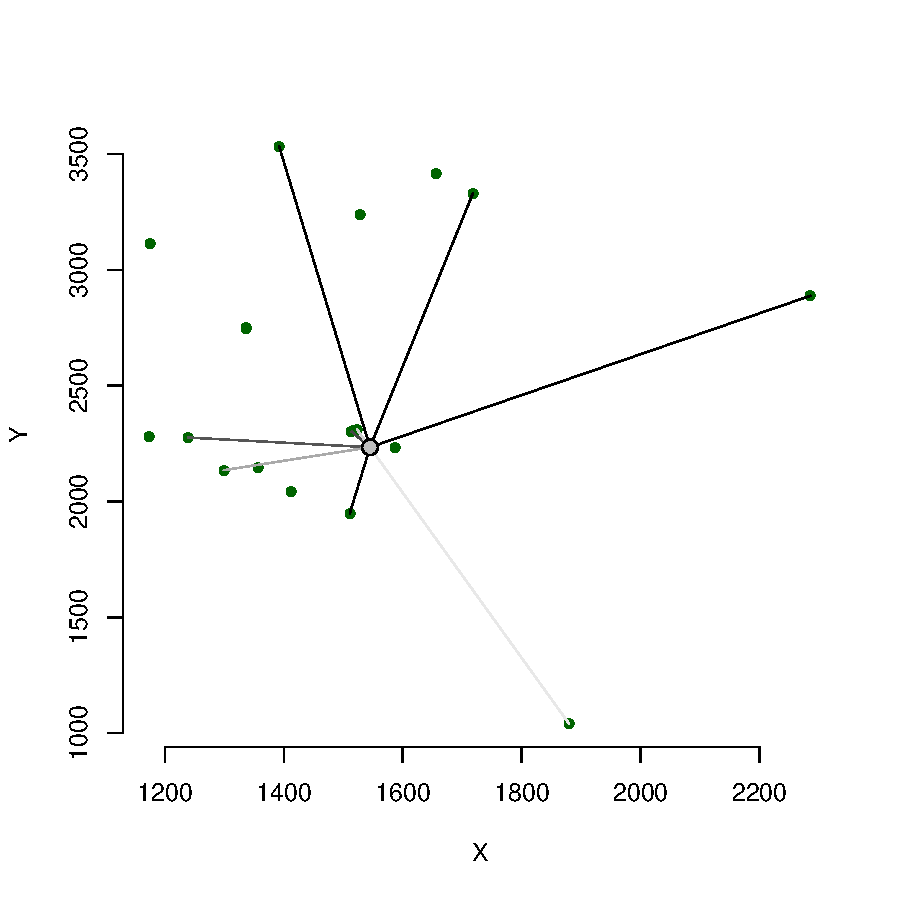
\includegraphics{gstudio-061}
	\caption{Spatial pattern of parentage for family 474 in the \emph{Cornus florida} dataset.  Darkness of the lines indicated fractional paternity (light=less, darker=greater).}
\end{figure}


\chapter{Population Graphs}

\section{Synopsis}

A population graph is a topological representation of within and among population genetic variance first introduced by Dyer \& Nason (2004).  It is particularly well suited to characterizing how spatial genetic variation is distributed among sites.

\begin{Schunk}
\begin{Sinput}
> require(gstudio)
> data(araptus_attenuatus)
> baja <- araptus_attenuatus[araptus_attenuatus$Species != "CladeB",]
\end{Sinput}
\end{Schunk}

\section{Simple Population Graphs}



\begin{Schunk}
\begin{Sinput}
> graph <- population.graph(baja,"Pop")
\end{Sinput}
\begin{Soutput}
tranforming data... done
Rotating mv genos and partitioning...  done
Estimating conditional genetic covariance... done
Making graph... done
\end{Soutput}
\begin{Sinput}
> summary(graph)
\end{Sinput}
\begin{Soutput}
Vertices: 36 
Edges: 59 
Directed: FALSE 
No graph attributes.
Vertex attributes: name, size, color.
Edge attributes: weight.
\end{Soutput}
\begin{Sinput}
> l <- layout.fruchterman.reingold(graph)
> plot(graph,layout=l,vertex.label=V(graph)$name)
\end{Sinput}
\end{Schunk}
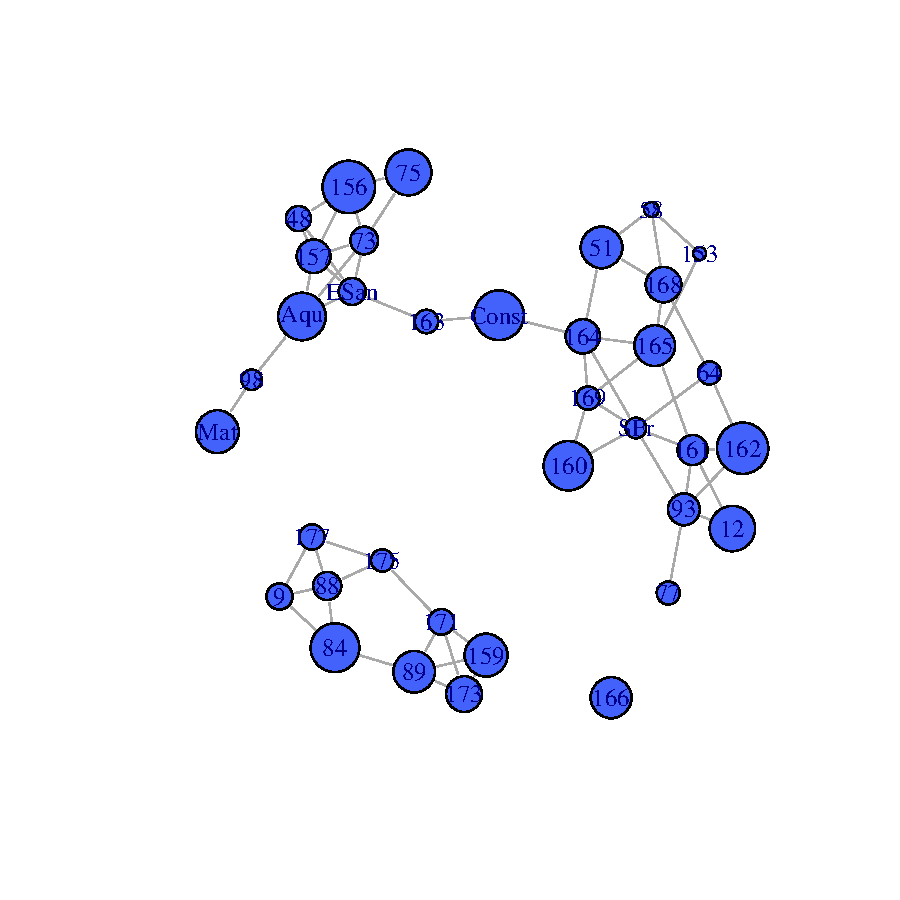
\includegraphics{gstudio-063}

We know that these data are a mixture of two putative species denoted as \texttt{CladeA} and \texttt{CladeC}.  

\begin{Schunk}
\begin{Sinput}
> table(baja$Species)
\end{Sinput}
\begin{Soutput}
CladeA CladeC 
    75    252 
\end{Soutput}
\end{Schunk}

We can color the nodes depending upon the identity of clade representation at the node-level.  If there is a mixture of species, you would expect to find that the mixed populations would be topologically intermediate between populations made up of pure samples.

\begin{Schunk}
\begin{Sinput}
> getCladeColor <- function(pop,data) {
+ 	inds <- data$Species[data$Pop==pop]
+ 	levels.inds <- levels(as.factor(as.character(inds)))
+ 	if(length(levels.inds)==2) return("red")
+ 	else if( levels.inds=="CladeA" ) return("blue")
+ 	else return("green")
+ }
> colors <- unlist(lapply(V(graph)$name, function(x) getCladeColor(x,baja)))
> plot(graph,layout=l,vertex.label=V(graph)$name,vertex.color=colors)
\end{Sinput}
\end{Schunk}
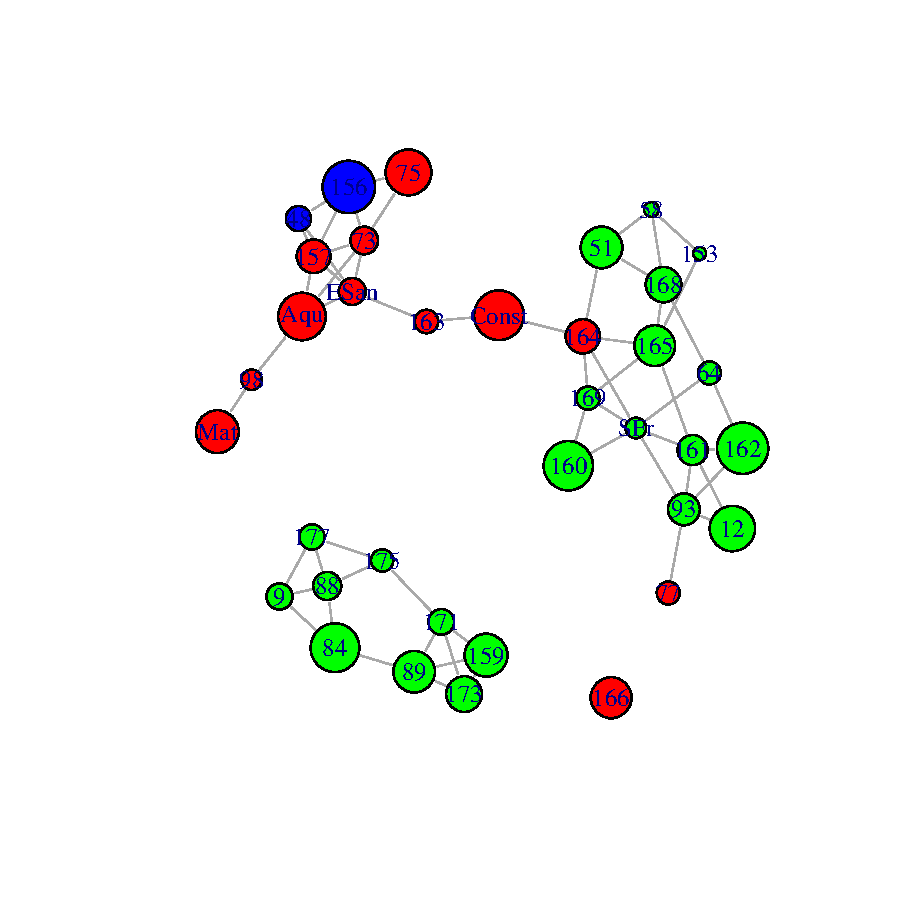
\includegraphics{gstudio-065}


So if we only use the samples from \texttt{CladeC} we may be actually analyzing the data in a way that makes sense.  Do this by:

\begin{enumerate}
	\item Use only the \texttt{CladeC} individuals
	\item Get rid of the populations with say $N<5$ individuals
	\item Make graph and examine the topology
\end{enumerate}


\begin{Schunk}
\begin{Sinput}
> baja.cladeC <- baja[baja$Species=="CladeC",]
> inds.per.pop <- lapply( partition(baja.cladeC,"Pop"), function(x) dim(x)[1] )
> ## Examine inds per pop to figure out which have <5 individuals save in smPops
> smPops <- c("Const","ESan","157","73","Aqu","Mat","98","75")
> baja.cladeC <- baja.cladeC[ !(baja.cladeC$Pop %in% smPops) , ]
> graph.cladeC <- population.graph(baja.cladeC,"Pop")
\end{Sinput}
\begin{Soutput}
tranforming data... done
Rotating mv genos and partitioning...  done
Estimating conditional genetic covariance... done
Making graph... done
\end{Soutput}
\begin{Sinput}
> summary(graph.cladeC)
\end{Sinput}
\begin{Soutput}
Vertices: 26 
Edges: 33 
Directed: FALSE 
No graph attributes.
Vertex attributes: name, size, color.
Edge attributes: weight.
\end{Soutput}
\begin{Sinput}
> l <- layout.fruchterman.reingold(graph.cladeC)
> plot(graph.cladeC,layout=l,vertex.label=V(graph.cladeC)$name)
\end{Sinput}
\end{Schunk}
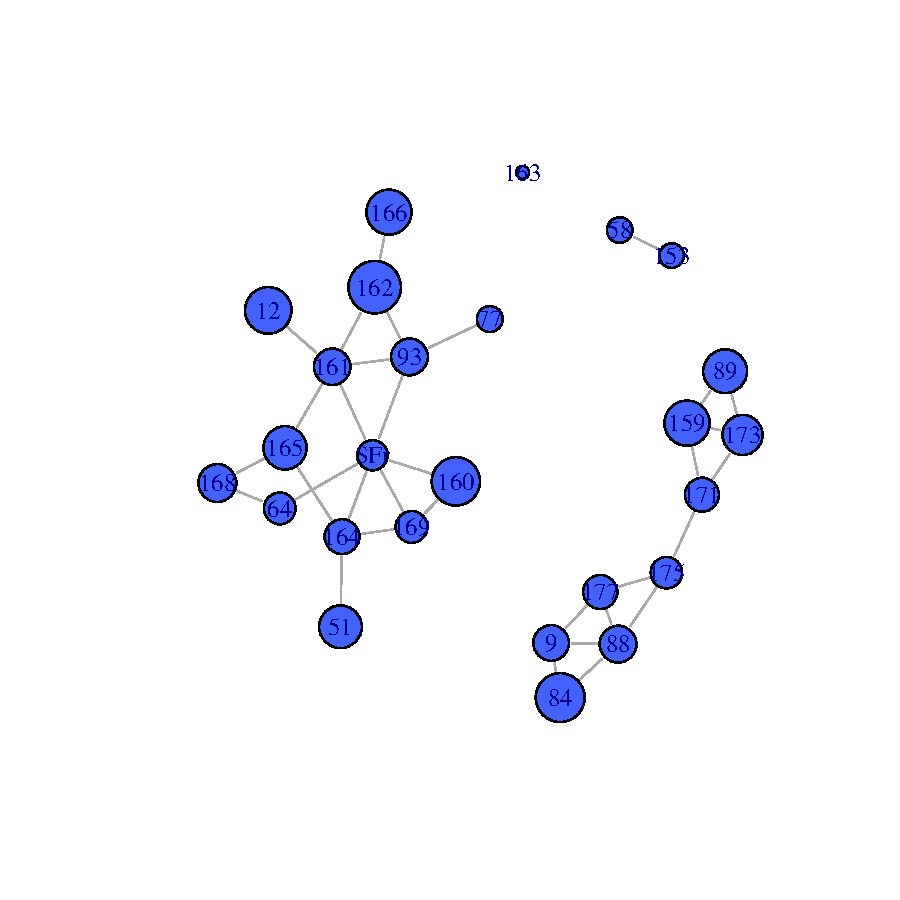
\includegraphics{gstudio-066}

From this plot, you can see even when we only focus on the true \texttt{CladeC} individuals, there is still partitioning of genetic covariance!  


\section{Node Position}

Both node and edge position in the topology can easily be determined using common network analysis tools.  The \texttt{igraph} package has some as does the most excellent \texttt{sna} package.  Here is a quick example where the size of the node is depicting the node's betweeness (e.g., the number of shortest paths that go through that node).

\begin{Schunk}
\begin{Sinput}
> pop.betweenness <- betweenness(graph.cladeC,directed=F)
> plot(graph.cladeC,layout=l,vertex.label=V(graph.cladeC)$name,vertex.size=pop.betweenness)
\end{Sinput}
\end{Schunk}
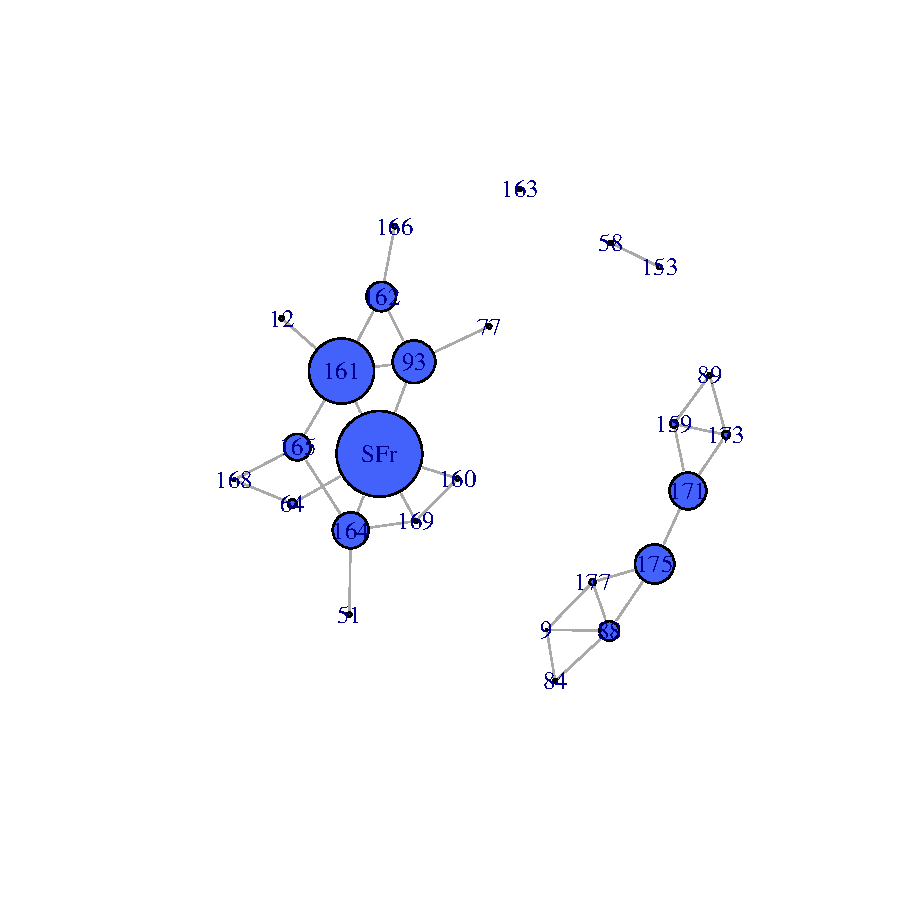
\includegraphics{gstudio-067}

Which is rather interesting since betweenness can be used to classify relative population importance.  Presently, it is common to use genetic diversity as a surrogate to identify populations of high conservation importance, but betweenness relates to the connectivity of the gene flow topology on the landscape and is not necessarily correlated with genetic diversity.

\begin{Schunk}
\begin{Sinput}
> cor.test(V(graph.cladeC)$size,pop.betweenness,method="spearman")
\end{Sinput}
\begin{Soutput}
	Spearman's rank correlation rho

data:  V(graph.cladeC)$size and pop.betweenness 
S = 3259.634, p-value = 0.5779
alternative hypothesis: true rho is not equal to 0 
sample estimates:
       rho 
-0.1144049 
\end{Soutput}
\end{Schunk}


\section{Conditional Genetic Distance}

In Dyer \emph{et al.} (2010) we showed that graph distance (e.g., the shortest path connecting points in the topology) was more powerful than pair-wise structure and distance approaches.  We denoted the among population distance as $cGD$ for conditional graph distance.

Since this topology is disconnected, we'll just focus on the medium sized component, the one with \texttt{84} in it.

\begin{Schunk}
\begin{Sinput}
> connected.to.84 <- subcomponent(graph.cladeC,v="84")
> med.graph <- subgraph(graph.cladeC,v=connected.to.84)
> med.layout <- layout.fruchterman.reingold(med.graph)
> plot(med.graph,layout=med.layout,vertex.label=V(med.graph)$name)
> D <- shortest.paths(med.graph)
\end{Sinput}
\end{Schunk}
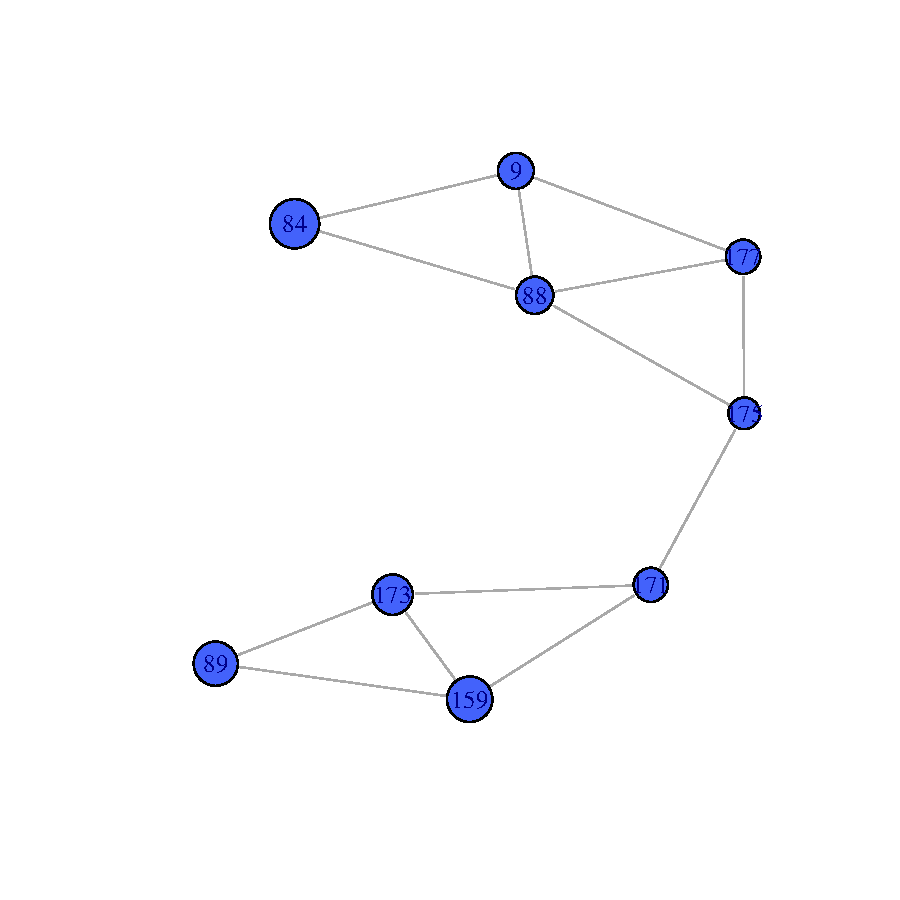
\includegraphics{gstudio-069}

As discussed previously, we can also get the pair-wise physical distance and then examine "Isolation by Graph Distance" (IBGD), which has some nice properties that make it perhaps more precise than IBD based upon pair-wise structure estimates.

\begin{Schunk}
\begin{Sinput}
> pops <- V(med.graph)$name
> P <- stratum.distance(baja.cladeC,"Pop",lat="Lat",lon="Long",subset=pops)
> plot(D[lower.tri(D)] ~ P[lower.tri(P)], bty="n",xlab="Physical Distance",ylab="Graph Distance")
\end{Sinput}
\end{Schunk}
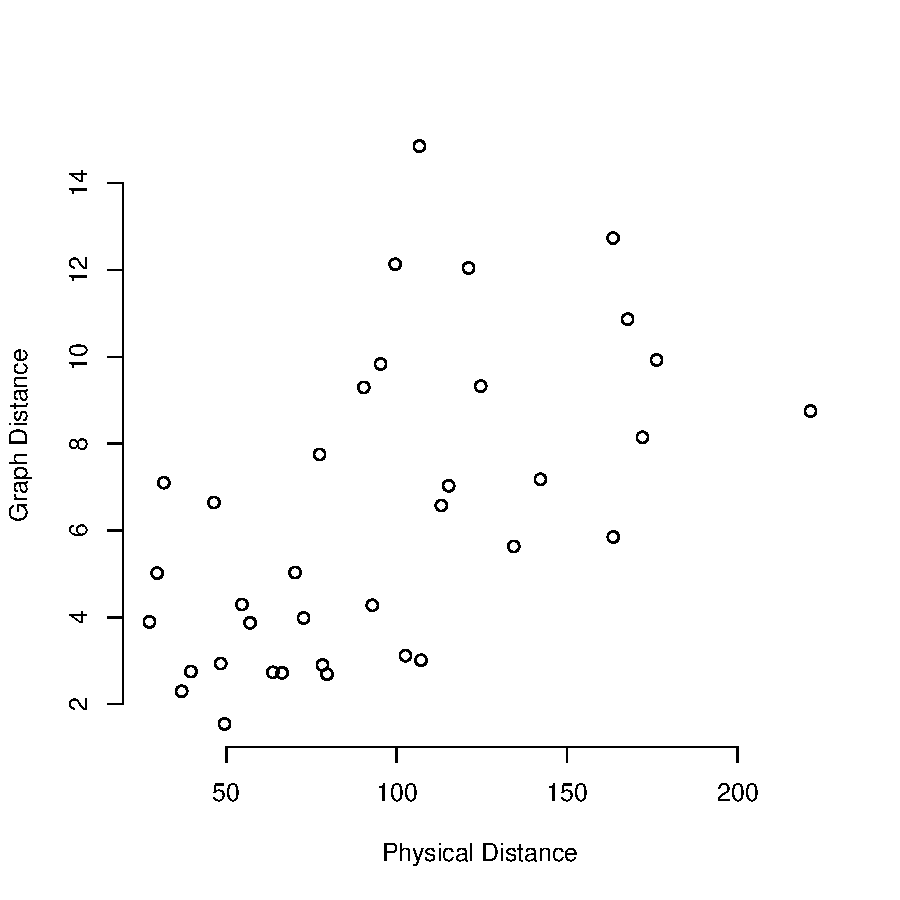
\includegraphics{gstudio-070}


We can use a Mantel test to see if there is a correlation between graph and physical distance for this subcomponent.

\begin{Schunk}
\begin{Sinput}
> require(ecodist,quietly=T)
> mantel(as.dist(D)~as.dist(P)) ##pval3 is Ho: Mantel-R=0
\end{Sinput}
\begin{Soutput}
   mantelr      pval1      pval2      pval3  llim.2.5% ulim.97.5% 
 0.5687480  0.0090000  0.9920000  0.0090000  0.4824620  0.7026195 
\end{Soutput}
\end{Schunk}

The \texttt{pval3} is the probability of $H_O: Mantel\rho=0 $.  


\section{Graph Partitions}

A very important point needs to be made here regarding subgraphs and partitions of the whole data set.  The disconnected subgraph in the previous section is not necessarily the same graph you would get if you partitioned the genotypes into only those populations and then make the graph.  Compare the previous network topology to this one.

\begin{Schunk}
\begin{Sinput}
> tmp.pop <- baja[baja$Pop %in% c("9","84","88","89","159","171","173","175","177")]
> tmp.graph <- population.graph(tmp.pop,"Pop")
\end{Sinput}
\begin{Soutput}
tranforming data... done
Rotating mv genos and partitioning...  done
Estimating conditional genetic covariance... done
Making graph... done
\end{Soutput}
\begin{Sinput}
> plot(tmp.graph,layout=med.layout,vertex.label=V(tmp.graph)$name)
\end{Sinput}
\end{Schunk}
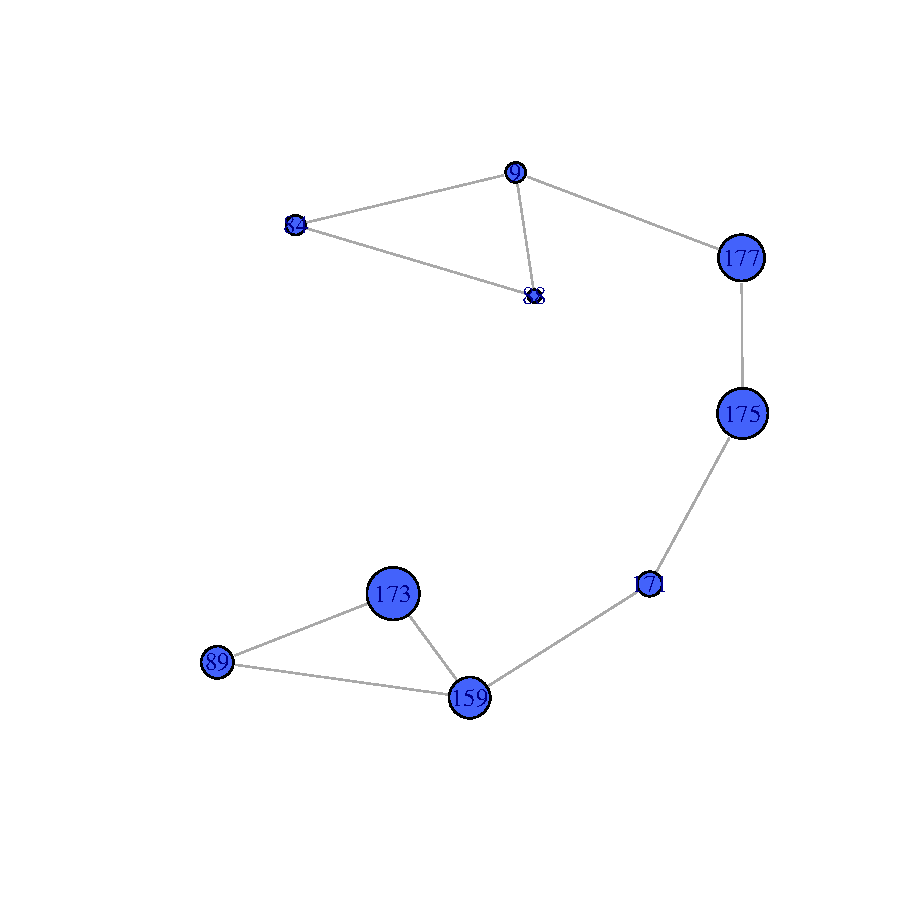
\includegraphics{gstudio-072}

This is because Population Graphs are constructed using \emph{Conditional Genetic Covariance}.  The genetic covariance between populations \texttt{173} \& \texttt{171} is conditional on the their covariance with all the other data in the data set.  In the first graph this includes the populations in this subgraph as well as the populations outside the subgraph.  
%
%  GStudio Documentation: GStudioMapping
%
%  Created by dyer on 2011-07-20.
% \documentclass[letterpaper]{article}
% \usepackage[margin=1in]{geometry}
% \usepackage{Sweave}
% \usepackage[parfill]{parskip}
% \usepackage{color}


\chapter{Mapping Population Genetic Data}

\section{Synopsis}

This vignette goes over some of the methodologies available for creating google KML files to display aspects of genetic data in either Google Earth, Google Maps, or even as an import into Arc.  These functions are part of an extension package \texttt{gstudio-sp} that extends the \texttt{gstudio} package by adding spatial components. They are kept separate from the rest of the \texttt{gstudio} package because one may not need to use the spatial components every time.

Here the \emph{Araptus attenuatus} data set will be used and in particular the subset of populations that formed the disconnected subgraph in the \emph{Population Graphs} vignette from the \texttt{gstudio} package.

\begin{Schunk}
\begin{Sinput}
> require(gstudio)
> data(araptus_attenuatus)
> popsToKeep <- c("88","9","84","177","175","173","171","89","159")
> baja <- araptus_attenuatus[araptus_attenuatus$Pop %in% popsToKeep]
\end{Sinput}
\end{Schunk}


\section{Pies On Maps}

Often it is of interest to look at global changes in allele frequencies.  While it is true that the frequency of an allele or set of alleles can be plot as a function of latitude or longitude, there is also value in putting it on a map. The function \texttt{pies.on.map} takes a \texttt{Population} file, a stratum, a list of loci, and some coordinate names in the population.  In most of the functions in \texttt{spgen} if you have your latitude and longitude variables labeled "Latitude" and "Longitude", you do not need to specify them in the function call. 

\begin{Schunk}
\begin{Sinput}
> pies.on.map(filename="~/Desktop/Baja.pies.kml",pop=baja,stratum="Pop",loci=c("EN","LTRS"),lat="Lat",lon="Long")
\end{Sinput}
\end{Schunk}

This creates a KML file that you can open in Google Earth and looks something like Figure \ref{fig:baja.pies}

\begin{figure}[p]
	\centering
	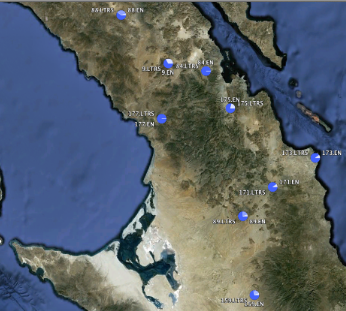
\includegraphics{baja_pies}
	\caption{Allele frequencies for locus 'EN' in \emph{Araptus attenuatus}.}
	\label{fig:baja.pies}
\end{figure}

\clearpage
\section{Population Graphs On Maps}

It is also helpful to put graph topologies on a map.  Here a population graph is created using the wrapper function \texttt{spatial.population.graph}.  This function adds latitude, longitude, and colors as properties to a normal population graph and is required for spatial plotting.  You can add these properties yourself if you like (use the \texttt{list.vertex.properties} function to see what is different) to a normal graph or you can just make the graph using this function.

\begin{Schunk}
\begin{Sinput}
> graph <- spatial.population.graph(pop="baja",stratum="Pop",lat="Lat",lon="Long")
> popgraph.on.map(graph,filename="~/Desktop/popgraph.on.map.kml")
\end{Sinput}
\end{Schunk}

\begin{figure}[h]
	\centering
	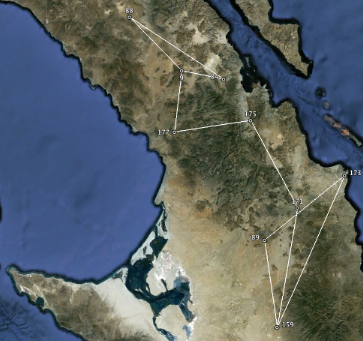
\includegraphics{baja_graph}
	\caption{Population graph for the northern group of \emph{Araptus attenuatus} populations.}
	\label{fig:baja.graph}
\end{figure}


\backmatter

\chapter{Bibliography}

Bray JR, Curtis JT.  1957.  An ordination of upland forest communities of southern Wisconsin. \emph{Ecological Monographs} {\bf 27}:325-349.

Cavalli-Sforza LL, Edwards AWF. 1967. Phylogenetic analysis: models and estimation procedures. \emph{American Journal Human Genetics}, \textbf{19}, 233-257.

Dyer RJ, Nason JD. 2004.  Population Graphs: The graph-theoretic shape of genetic structure. \emph{ Molecular Ecology}, \textbf{13}, 1713-1728.

Dyer RJ, Nason JD, Garrick RC.  2010.  Landscape modeling of gene flow: Improved power using conditional genetic distance derived from the topology of population networks.  \emph{Molecular Ecology}, \textbf{19}, 3746-3759.

Smouse, PE and R Peakall (1999)  Genetics

\printindex


\end{document}
